\documentclass[%
11pt,%
twoside,%
titlepage,%
german,%
headsepline%
]{scrartcl}

\usepackage{lastpage}
\usepackage{geometry}
\usepackage{graphicx}
\usepackage[utf8]{inputenc}
\usepackage[ngerman]{babel}
\usepackage{lscape}
\usepackage[framemethod=TikZ]{mdframed}
\usepackage[most]{tcolorbox}
\usepackage{mymath}
\usepackage{units}
\usepackage{nicefrac}
\usepackage{pgf,tikz}
\usetikzlibrary{arrows}
\usepackage{colortbl}
\usepackage{hhline}
\usepackage{multirow}
\usepackage[extendedchars]{grffile}
\usepackage{caption}
\usepackage{multicol,calc}
\usepackage{blindtext}
\usepackage{pdfpages}
\usepackage{hyperref}
%\usepackage[official]{eurosym}
\usepackage{framed}
\usetikzlibrary{arrows}
\usetikzlibrary{positioning}
\usetikzlibrary{shadows}

\usepackage{marginnote}
\usepackage{qrcode}
\qrset{height=9ex}

\usepackage{longtable}
\usepackage{listings}
\usepackage{wrapfig}


% Command, um Tabellen-Spalten anzupassen
\newcommand{\spaltenheight}{\rule{0mm}{3ex}}
\newcommand{\spaltenwidth}{\rule{3cm}{0mm}}
\newcommand{\spaltensep}{\\[1ex]}
%\arrayrulecolor{darkgreen}
\doublerulesepcolor{white}
\definecolor{lightyellow}{rgb}{1,1,0.8}
\definecolor{Gray}{gray}{0.9}


% Pagestyle/Layout
%\geometry{a4paper , tmargin =2.5cm,	bmargin=3cm, lmargin =2.5cm,	rmargin =2.5cm,	headheight=3em, headsep=1em, footskip=1cm}
\setlength{\parindent}{0pt} \setlength{\parskip}{1em}
%für TwoSide
%\lehead{\headmark\pagemark}
%\cehead{}
%\rehead{}
%\lohead{}
%\cohead{}
%\rohead{\headmark}
%für OneSide
%\ihead{}
%\chead{}
%\ohead{}
%\setheadsepline{0.5pt} % Linie zur Begrenzung
%\setfootsepline{0.5pt} % Linie zur Begrenzung
\pagestyle{headings} % gemachte Einstellungen anwenden


\subject{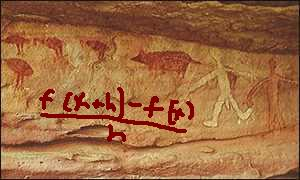
\includegraphics[width=0.618\textwidth]{pictures/cave.jpg}}
\title{Differentialrechnung}
\subtitle{The Core of the Whole Business}
\author{}
\date{}


\begin{document}
\maketitle
\tableofcontents
\cleardoublepage

\section{Tangenten- und Fl\"achenproblem}
Die Mathematik der Antike hat ihrer Nachwelt zwei klassische Probleme \"uberliefert: das \emph{Tangentenproblem} und das \emph{Fl\"achenproblem}.

\begin{itemize}
\item Die Konstruktion einer Tangente an einen Kreis ist relativ einfach. Sie versagt aber schon, wenn man versucht, eine Tangente an eine Ellipse zu konstruieren. Die griechischen Geometer hatten f\"ur die Ellipse ein neues Verfahren erdacht, das aber schon wieder bei einer anderen Kurve, der Parabel, versagte. Die Konstruktion der Parabeltangente liess sich nicht auf die Hyperbel \"ubertragen; man musste also f\"ur jede Kurve eine ganz neue Konstruktion ersinnen. Wenn nur wenige Kurven bekannt sind, besteht kein Anlass, nach einer allgemeinen Methode zu suchen. Die Situation \"anderte sich aber schlagartig, als zu Beginn des 17. Jahrhunderts die analytische Koordinatengeometrie entstand und somit beliebig viele Kurven zu untersuchen waren. Jetzt wurde eine universelle Methode verlangt, die es erm\"oglicht, den Verlauf der Tangente f\"ur jede beliebige Kurve zu studieren.
\end{itemize}

\begin{itemize}
\item Das Fl\"achenproblem bestand darin, den Inhalt einer durch Kurven begrenzten Fl\"ache zu berechnen. Zu diesem Problem leistete vor allem \textsc{Archimedes} (287 -- 212 v.u.Z) Hervorragendes. Seine Methode, die Exhaustionsmethode, bestand darin, die zu berechnende Fl\"ache durch eine Folge von Fl\"achen mit schon bekanntem Inhalt auszusch\"opfen. Wenn man das Fl\"achenproblem gel\"ost hat, f\"allt die Berechnung des Volumens eines K\"orpers nicht mehr so schwer. Viele spezielle Fl\"achen und K\"orper konnten so durch teilweise raffinierte Zerlegungen berechnet werden. Aber es existierte noch keine universelle Methode.
\end{itemize}

\section{Durchschnittliche \"Anderungsrate}
\textsc{Heraklit} (535 -- 475 v.u.Z) soll gesagt haben: \glqq alles bewegt sich fort\grqq; \textsc{Aristoteles} (384 -- 322 v.u.Z) schrieb \"uber \textsc{Heraklit} und seine Anh\"anger:
\begin{quote}
\glqq\dots diese aber sagen, dass alles andere im Werden und im Fluss sei.\grqq
\end{quote}

Nichts entgeht der Ver\"anderung. Alles w\"achst oder schrumpft, erw\"armt sich oder k\"uhlt sich ab, wechselt die Stellung, die Farbe oder die Zusammensetzung. Die Fauna und die Flora liefern beliebig viele Beispiele, selbst Felsen dehnen sich in der Sonne aus und ziehen sich im Schatten zusammen. K\"orpergr\"osse, K\"orpertemperatur, Pulsfrequenz, Blutdruck sind einige Beispiele f\"ur --- direkt auf den Menschen --- bezogene Gr\"ossen, die sich mit der Zeit \"andern.

Der Mathematik der Antike gelang es nicht, ver\"anderliche Gr\"ossen mathematisch zu erfassen. Ihre Mathematik war, bis auf wenige Ausnahmen, eine feste und stillstehende Welt. Andererseits zeigt dies, dass es sehr schwer ist, einen Ver\"anderungsprozess zu analysieren und das dahinterstehende Naturgesetz zu finden.

Erst im 16. und 17. Jahrhundert war die Zeit reif, den allgemeinen Begriff der ver\"anderlichen Gr\"osse in die Mathematik aufzunehmen.
Was waren die Triebfedern f\"ur diese Entwicklung?

F\"ur die Anwendungen der Mathematik standen Probleme der Geod\"asie, der Astronomie, des Artilleriewesens, der Schifffahrt, des Kanalbaus, der maschinellen Ausr\"ustung von Manufakturen im Vordergrund. Insbesondere wurden beispielsweise gebraucht: Maschinen zur Wasserhaltung und F\"orderung in Bergwerken, Maschinen zur Textil- und Papierherstellung, Maschinen f\"ur den Tunnelbau, Schiffshebewerke, Kr\"ane etc.. Die Uhren mussten enorm verbessert werden. \textsc{Leonardo da Vinci} machte sich sogar schon Gedanken \"uber Flugmaschinen, Unterseeboote und Wagen, die ohne Zugtiere fahren konnten.
Die Mathematik sollte vor allem mechanische Bewegungsabl\"aufe --- Planetenbewegungen, Fallbewegungen, Bewegungen gegeneinander beweglicher Maschinenteile --- erfassen und theoretisch beschreiben k\"onnen.
Der neuen Mathematik des 16. und 17. Jahrhunderts gelang es, mit denselben Methoden sowohl das Tangentenproblem als auch das Fl\"achenproblem, als auch die Bewegungsprobleme zu l\"osen! Sie konnte gleichzeitig die Verwandtschaft und die Gleichartigkeit all dieser Probleme aufzeigen. Auf diesen L\"osungen aufbauend konnten weitere Probleme, die die naturwissenschaftliche Entwicklung immer weiter vorantrieben, bew\"altigt werden.
\textsc{Ren\'e Descartes} (1596 -- 1650) gelang es, die gegenseitige Abh\"angigkeit von ver\"anderlichen Gr\"ossen --- ausgedr\"uckt durch eine Gleichung oder eine Funk\-tion --- in einem Koordinatensystem graphisch darzustellen.
Weiterhin konnten die einzelnen Zust\"ande einer Bewegung sichtbar gemacht und genau studiert werden.
Es fehlte aber noch die klare Erfassung des Funk\-tions\-begriffes und eine auf ver\"anderliche Gr\"ossen zugeschnittene Rechentechnik. Der Funktionsbegriff erweist sich aus heutiger Sicht als fundamental, da durch ihn die gegenseitige Abh\"angigkeit der Gr\"ossen ausgedr\"uckt werden kann.
In der zweiten H\"alfte des 17. Jahrhunderts schufen dann \textsc{Isaac Newton} (1643 -- 1727) und \textsc{Gottfried Wilhelm Leibniz} (1646 -- 1716) unabh\"angig voneinander etwas f\"ur die bisherige Mathematik v\"ollig Neues, das die analytische Koordinatengeometrie von \textsc{Descartes} mit der von \textsc{Archimedes} stammenden Exhaustionsmethode verband.

\begin{figure}
\begin{center}
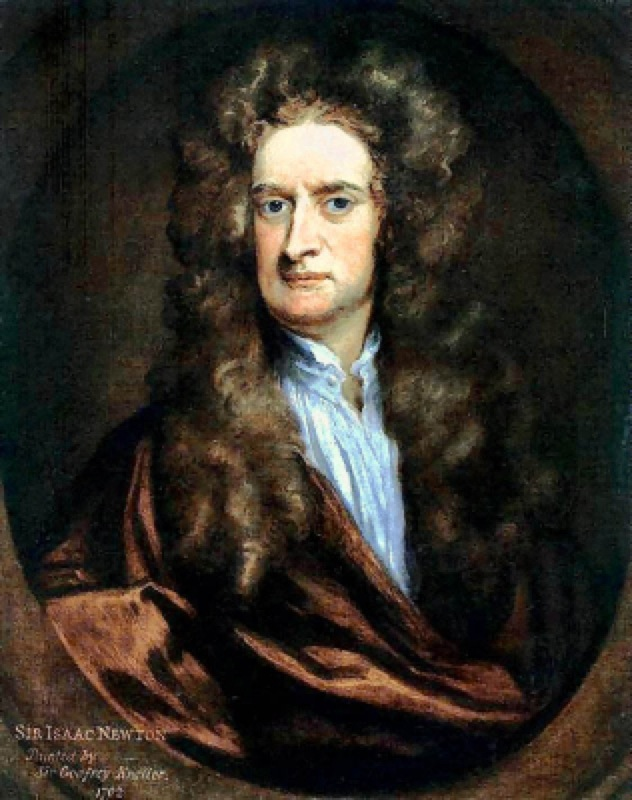
\includegraphics[width=0.4\textwidth]{pictures/newton}\hspace*{0.062\textwidth}
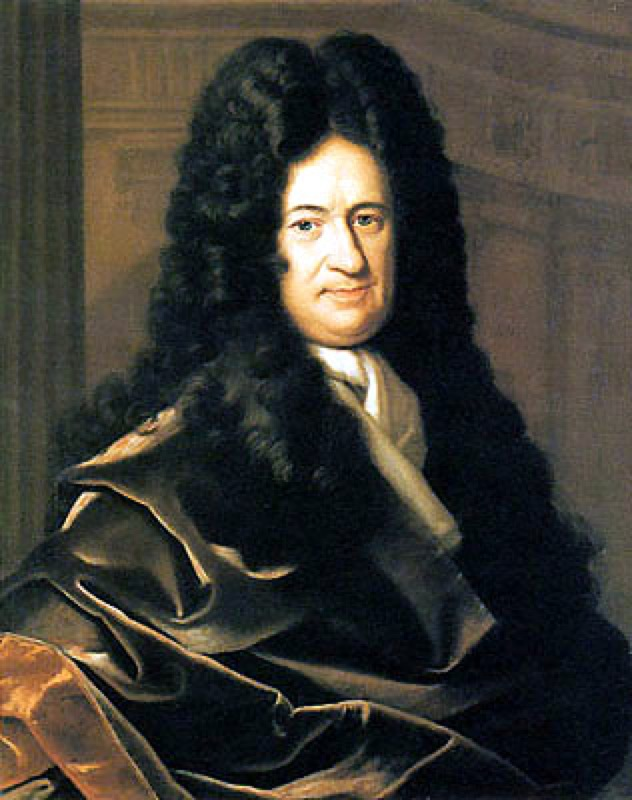
\includegraphics[width=0.4\textwidth]{pictures/leibniz}
\caption{\textsc{Sir Isaac Newton} und \textsc{Gottfried Wilhelm Leibniz}}
\end{center}
\end{figure}
Dieses neue Gebiet der Mathematik heisst heute Infinitesimalrechnung oder \emph{Analysis} oder Differenzial- und Integralrechnung oder im englischen Sprachraum \emph{Calculus}.

Die Differenzialrechnung, die das Tangentenproblem l\"ost, bildet unter anderem die Grundlage der mechanischen Bewegungen. Mit ihr kann beispielsweise der Physiker oder Techniker aus einer gegebenen Bahnkurve f\"ur jeden Zeitpunkt die augenblickliche Geschwindigkeit ermitteln. Sp\"ater eroberte sich die Differenzialrechnung immer mehr Anwendungsgebiete; zum Beispiel ist sie f\"ur die heutigen Wirtschaftswissenschaften unentbehrlich geworden.

Mit der Integralrechnung, die das Fl\"achenproblem l\"ost, konnte man bald nach ihrer Entdeckung auch die Bogenl\"ange eines Kurvenst\"uckes oder den Rauminhalt und die Oberfl\"ache eines krummfl\"achig begrenzten K\"orpers berechnen, aber auch viele physikalische Begriffe, wie zum Beispiel Schwerpunkt, Tr\"agheitsmoment, Arbeit etc. mathematisch erfassen. Als besonders n\"utzlich erwies sich die Integralrechnung zu der Zeit, als die Kohle als Energiequelle die Arbeit des Menschen und des Lasttiers zu ersetzen begann. Mit ihr konnte man n\"amlich die Leistung und den Wirkungsgrad von Maschinen berechnen. Sp\"ater wurde die Integralrechnung auch zur Grundlage der Chemie der Energiestoffe (Thermodynamik).

Die Infinitesimalrechnung erlaubt es, \glqq Bewegungen abzustoppen\grqq\ und Augenblick f\"ur Augenblick zu analysieren. Sie ist neben der Wahrscheinlichkeitsrechnung und Statistik f\"ur die angewandten Naturwissenschaften auch heute noch der wichtigste Zweig der Mathematik. Jedes moderne Verkehrsmittel, jedes Fernsehger\"at, jede gr\"ossere Br\"ucke oder Maschine in einer Fabrik, aber auch leider jede Atombombe w\"are ohne Infinitesimalrechnung nicht denkbar.

Vom 17. Jahrhundert an ist es ein typisches mathematisches Problem, aufgrund einiger Daten oder Gleichungen eine Funktion zu finden, die verschiedene Bedingungen zu erf\"ullen hat. Die Theorie der Funktionen (Potenzreihenentwicklung) und die L\"osungen der entsprechenden Gleichungen (Differenzial- und Integralgleichungen) waren entscheidend f\"ur die Entwicklung der Naturwissenschaften, insbesondere der Physik. Mit der Zeit traten immer kompliziertere Funktionen, praktischen oder theoretischen Ursprungs, auf. Statt einer Funktion mit einer Variablen waren mehrere Funktionen mit mehreren Variablen und sie verbindende Differenzial- oder Integralgleichungen zu betrachten. Beispielsweise sind in der Hydrodynamik sich r\"aumlich ausdehnende Gase oder Fl\"ussigkeiten zu betrachten: Druck, Dichte und drei Geschwindigkeitskomponenten sind von Ort und Zeit abh\"angig, was ein System von f\"unf Funktionen mit vier Variablen ergibt.
Wenn es gelingt, die Parameter einer ver\"anderlichen Situation in Gleichungen auszudr\"ucken, kann man rein theoretisch und ohne Experimente mit der Infinitesimalrechnung die Naturgesetze herausfinden, denen die Parameter unterliegen.
\textsc{Bergamini} schreibt in seinem Buch \glqq Die Mathematik\grqq:
\begin{quote}
\glqq Die zu berechnenden Ver\"anderungen k\"onnen so dramatisch sein wie die steigende Geschwindigkeit einer Rakete nach dem Start oder so sanft wie die unterschiedlichen Steigungen einer modernen Bergstrasse. Sie k\"onnen so sichtbar sein wie die gewonnenen Pfunde auf einer einst schmalen Taille, aber auch so unsichtbar wie der Phasenwechsel in einem Stromkabel. H\"orbar k\"onnen sie sein wie das Crescendo einer \textsc{Beethoven}-Symphonie oder so schweigend wie die Wasserkraft hinter einem Damm. Sie sind jedenfalls berechenbar.\grqq
\end{quote}

\section{Momentane \"Anderungsrate}
Bei einer ver\"anderlichen Situation ist nicht nur der augenblickliche Zustand von Interesse; vielmehr interessiert oft, mit welcher Geschwindigkeit sich die Situation \"andert. F\"ur die Wettervorhersage ist nicht allein die Gr\"osse des Luftdrucks wichtig, sondern vor allem, wie stark der Druck je Stunde steigt oder f\"allt. F\"ur den Wirtschaftswissenschaftler ist neben dem Marktpreis eines Produktes von besonderer Wichtigkeit, wie schnell sich der Preis mit der Zeit \"andert (Teuerungsrate). F\"ur den Chemiker ist interessant, wie sich die Reaktionsgeschwindigkeit eines von der Temperatur abh\"angigen chemischen Prozesses ver\"andert, wenn man die Temperatur um einige Grade absenkt bzw. erh\"oht.
Die Infinitesimalrechnung von \textsc{Newton} und \textsc{Leibniz} kann diese und \"ahnliche Fragen mit zwei neuen Verfahren, der Differenziation und der Integration, beantworten.

Wir betrachten eine beliebige, zeitlich ver\"anderliche Situation, deren einzelne Zust\"ande durch die Funktion
$$f: t\mapsto f(t)$$
beschrieben werden k\"onnen. Man kann relativ einfach eine \emph{durchschnittliche} \"An\-derungs\-ge\-schwin\-dig\-keit des
Funktionswertes angeben, indem man die zu zwei bestimmten Zeitpunkten $t_1$ und $t_2$ gebildete Differenz der zugeh\"origen Funktionswerte $f(t_1)$ und $f(t_2)$ durch die Zeitspanne dividiert.
$$\overline{v}=\frac{\text{\"Anderung von }f(t)}{\text{\"Anderung von }t}=\frac{f(t_2)-f(t_1)}{t_2-t_1}=\frac{\Delta f}{\Delta t}$$
Mit der Differenziation kann man jedoch die \emph{momentane} \"An\-derungs\-ge\-schwin\-dig\-keit des Funktionswertes zu einem beliebigen Zeitpunkt $t$ berechnen.

Man bezeichnet \"ublicherweise einen Zuwachs der Variablen $t$ mit $\Delta t$ und die entsprechende \"Anderung des Funktionswertes zwischen den Zeitpunkten $t$ und $t+\Delta t$ mit $\Delta f$.
\begin{figure}
\centering
\definecolor{xdxdff}{rgb}{0.5,0.5,1}
\definecolor{ccqqqq}{rgb}{0.8,0,0}
\scalebox{1.3}{
\begin{tikzpicture}[line cap=round,line join=round,>=triangle 45,x=0.55cm,y=0.55cm]
\draw[->,color=black] (-0.72,0) -- (12.46,0);
\foreach \x in {,1,2,3,4,5,6,7,8,9,10,11,12}
\draw[shift={(\x,0)},color=black] (0pt,-2pt);
\draw[color=black] (12.18,0.08) node [anchor=south west] {$t$};
\draw[->,color=black] (0,-1.42) -- (0,4.6);
\foreach \y in {-1,1,2,3,4}
\draw[shift={(0,\y)},color=black] (2pt,0pt) -- (-2pt,0pt);
\draw[color=black] (0.1,4.2) node [anchor=west] {$y$};
\clip(-0.72,-1.42) rectangle (12.46,4.6);
\draw[line width=1.2pt,color=ccqqqq, smooth,samples=100,domain=-0.72:12.46] plot(\x,{0-(0.02)*(\x-2)*(\x+2)*(\x-11)});
\draw (2.0,3.3) node[anchor=north west] {$y=f(t)$};
\draw [dotted] (2.98,0.78)-- (3,0);
\draw (2.98,0.78)-- (9,0.8);
\draw [dotted] (9,0.8)-- (9,0);
\draw (2.7,0.02) node[anchor=north west] {$t$};
\draw (8.0,0.02) node[anchor=north west] {$t+\Delta t$};
\draw (5.82,0.9) node[anchor=north west] {$\Delta t$};
\draw (9,0.78)-- (9,3.08);
\draw (8.8,1.9) node[anchor=north west] {$\Delta f$};
\fill [color=xdxdff] (2.98,0.78) circle (1.5pt);
\fill [color=xdxdff] (9,3.08) circle (1.5pt);
\end{tikzpicture}
}
\caption{durchschnittliche Steigung $\frac{\gD f}{\gD t}$}
\end{figure}
Da Z\"ahler und Nenner jeweils Differenzen sind, heisst der Bruch Differenzenquotient. Jetzt braucht man nur zu verfolgen, was mit dem Bruch $\frac{\gD f}{\gD t}$ geschieht, wenn $\gD t$ gegen Null strebt. Zu Beginn gibt der Differenzenquotient die durchschnittliche \"Anderungsgeschwindigkeit des Funktionswertes zwischen den Zeitpunkten $t$ und $t+\gD t$ an. Wenn nun $\gD t$ gegen Null strebt, so strebt $\gD f$ auch gegen Null. Der Wert des Differenzenquotienten $\frac{\gD f}{\gD t}$ muss dabei nicht unbedingt gegen Null streben. Der Differenzenquotient hat, falls $\gD t$ gegen Null strebt, (hoffentlich!) einen Grenzwert. Dieser Grenzwert ist, falls er existiert, die augenblickliche \"Anderungsgeschwindigkeit des Funktionswertes zum Zeitpunkt $t$.
Man schreibt daf\"ur
$$\frac{\mathrm{d}f}{dt}=\lim_{\gD t\to0}\frac{\gD f}{\gD t}$$
und nennt diesen Grenzwert \emph{Differenzialquotient}.

Die Integration ist in gewisser Weise die Umkehrung der Differenziation, etwa in der Art, wie die Addition und Subtraktion oder Multiplikation und Division Umkehrungen voneinander sind. Bei der Integration sucht man eine Funktion, deren Differenzialquotient $q(t)$ bekannt ist. Man nennt diese Funktion das Integral von $q(t)$ und
schreibt
$$\int q(t)\,dt$$
(integrare: lat. wiederherstellen).
Kennt man zum Beispiel bei einer Autofahrt die zur\"uckgelegte Wegstrecke als Funktion der Zeit, so gibt der Differenzialquotient f\"ur einen bestimmten Zeitpunkt die momentane Geschwindigkeit an. Kennt man die Geschwindigkeit als Funktion der Zeit, so kann man mit Integration die zwischen zwei bestimmten Zeitpunkten zur\"uckgelegte Wegstrecke berechnen.

Die Differenziation hat lokalen Charakter, d.h. es gen\"ugt, die Funktion in einer beliebig kleinen Umgebung einer bestimmten Stelle zu kennen, um die \"Anderungsgeschwindigkeit an dieser Stelle zahlenm\"assig zu berechnen. Bei der Integration hingegen ist die Funktion als Ganzes von Bedeutung; deshalb ist bei der Integration ein anderer Grenzprozess erforderlich.

\begin{figure}
    \centering
    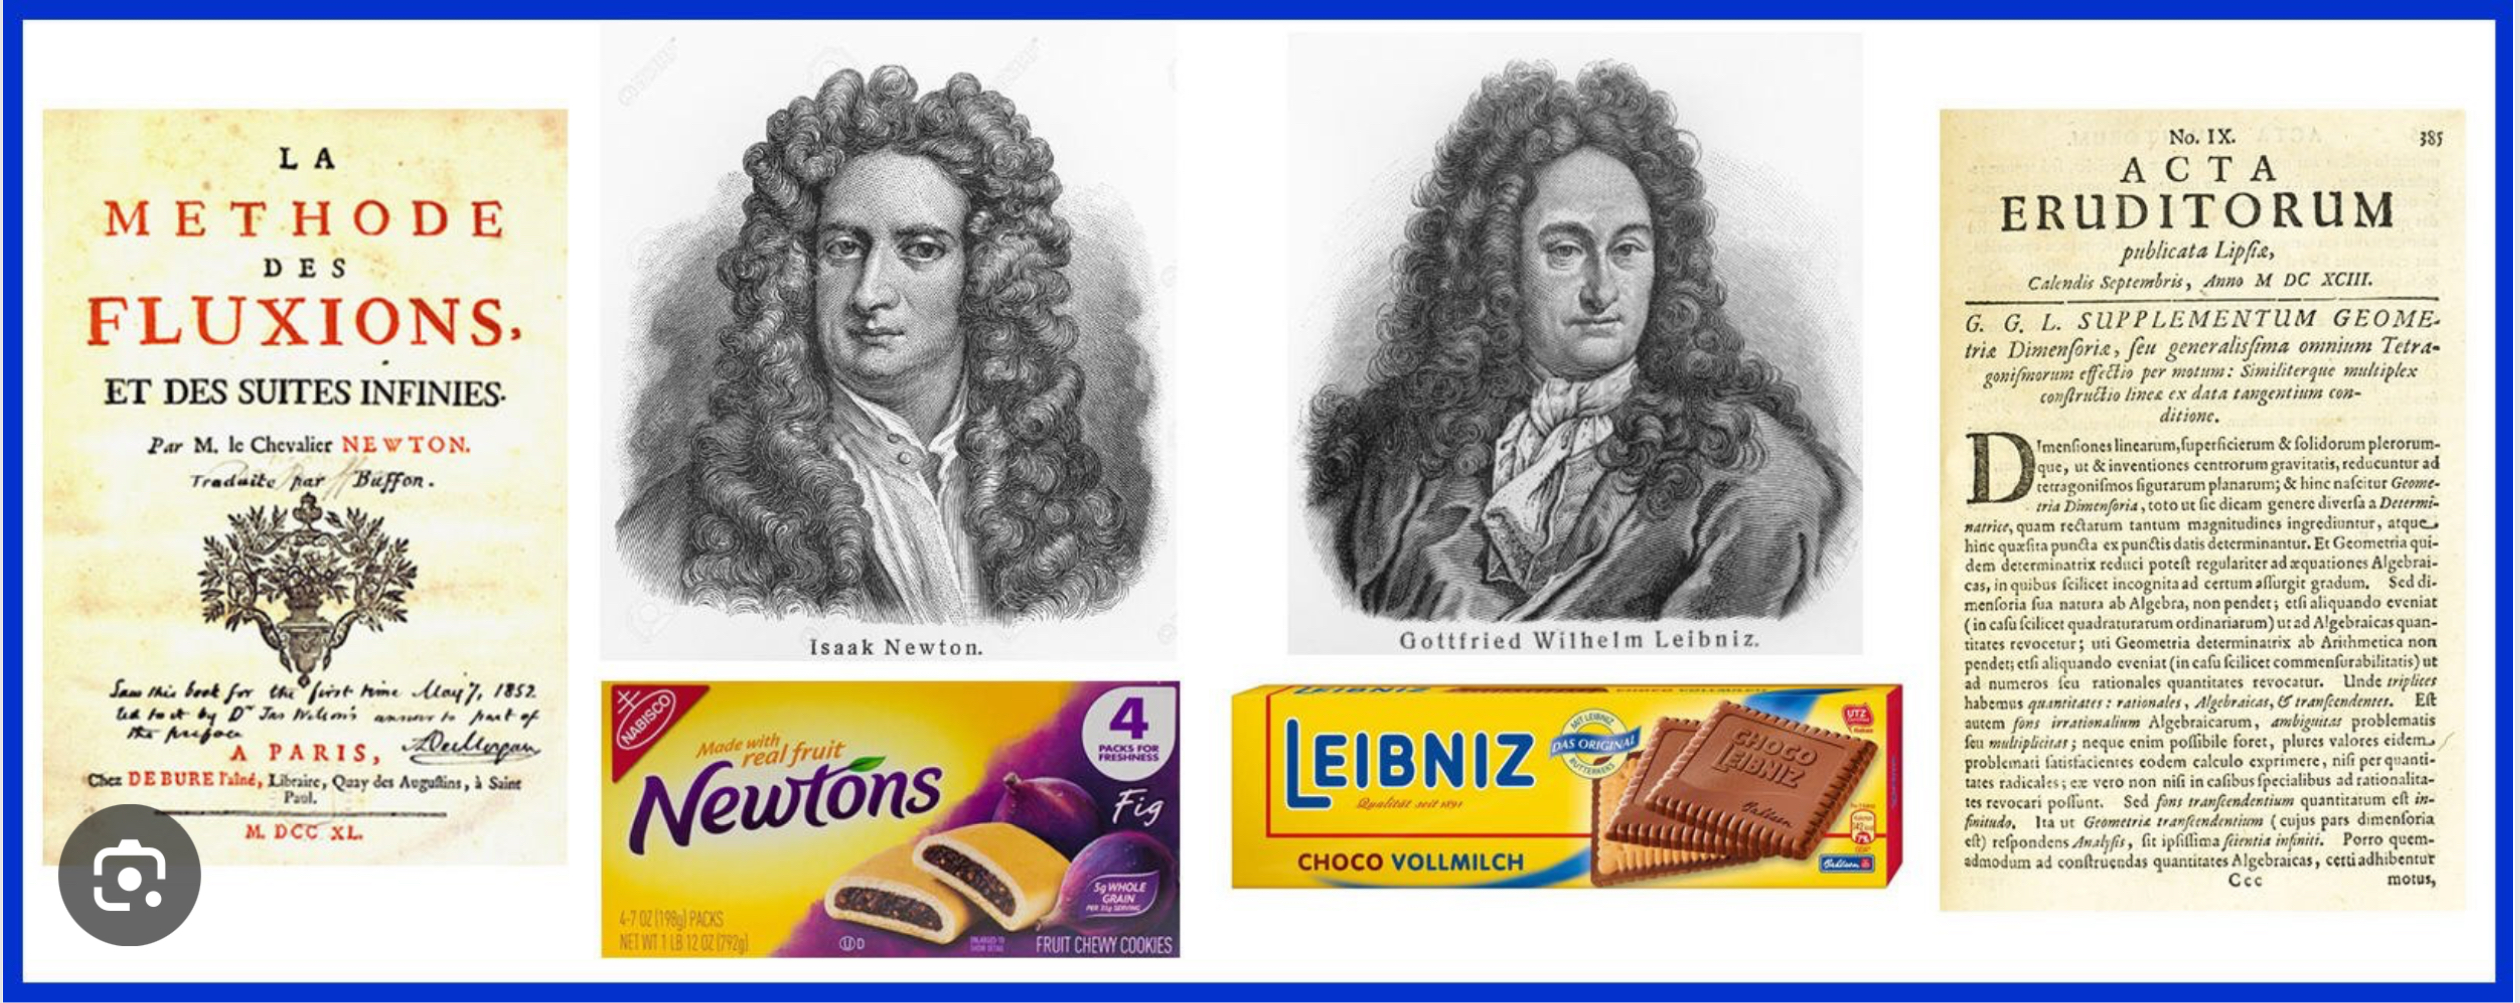
\includegraphics[width=0.62\textwidth]{pictures/newton_and_leibiz.jpeg}
    \caption{both have biscuits named after them}
    \label{fig:leibnizandnewton}
\end{figure}

Es mag vielleicht so aussehen, als ob \textsc{Newton} und \textsc{Leibniz} etwas Offensichtliches oder Selbstverst\"andliches entdeckt h\"atten. Viele Wissenschaftler hatten sich vor ihnen mit den gleichen Problemen besch\"aftigt, aber keiner konnte die einzelnen Erfolge zu einem Neuen und Einheitlichen zusammenf\"ugen. Differenziation und Integration konnten auf jede Art von ver\"anderlichen Gr\"ossen, wenn sie nur durch eine Gleichung miteinander verbunden werden konnten, angewendet werden. Es zeigte sich, dass die Differenzialrechnung das Tangentenproblem und die Integralrechnung das Fl\"achenproblem l\"osten. Tangenten- und Fl\"achenproblem erwiesen sich als zwei Seiten derselben M\"unze.
Nach der Entdeckung der Differenzial- und Integralrechnung steht nicht mehr das Einzelproblem im Vordergrund der Forschung, sondern die allgemeine Methode zur Erledigung ganzer Problemklassen. Das Einzelproblem wird zum \"Ubungsbeispiel degradiert. Ein neues, mit den vorhandenen Methoden nicht l\"osbares Einzelproblem veranlasst den Ausbau der Methoden, so dass es wieder zum \"Ubungsbeispiel wird. In der Mathematik wird so zuerst die grosse Entscheidung erkennbar, die auf anderen Gebieten erst 150 Jahre sp\"ater augenf\"allig wird, die Abkehr vom Handwerk und der Einzelanfertigung zur Maschinenarbeit und Serienfabrikation.

Nach jahrelangen Experimenten und vielen theoretischen Anl\"aufen konnte \textsc{Galilei} 1585 die Gesetze des freien Falls aufstellen: Ein auf die Erde herabfallender K\"orper legt in der Zeit t den Weg
$$s(t)=4.9 t^2$$
zur\"uck ($t$ in Sekunden, $s(t)$ in Meter); nach der Zeit $t$ hat der K\"orper die Geschwindigkeit
$$v(t)=9.8t$$
($v(t)$ in $\unitfrac{m}{s}$); seine Beschleunigung ist zu jedem Zeitpunkt konstant, n\"amlich
$$\unitfrac[9.8]{m}{s^2}$$
Mit der von \textsc{Newton} und \textsc{Leibniz} entdeckten Infinitesimalrechnung braucht man nur die Ausgangsfunktion
$$s:t\mapsto s(t)=4.9t^2$$
zu kennen. Die Geschwindigkeit ist die \"Anderung des Weges relativ zur Zeit, also der Differenzialquotient
$$\lim_{\gD t\to0}\frac{\gD s}{\gD t}=\lim_{\gD t\to0}\frac{4.9(t+\gD t)^2-4.9t^2}{\gD t}$$
und damit
$$v(t)=\lim_{\gD t\to0}4.9\cdot 2t+4.9\gD t=9.8t.$$
Die Beschleunigung $a(t)$ ist die Ver\"anderung der Geschwindigkeit relativ zur Zeit, also der Differenzialquotient
$$\lim_{\gD t\to0}\frac{\gD v}{\gD t}=\lim_{\gD t\to0}\frac{9.8(t+\gD t)-9.8t}{\gD t}=9.8$$
Die Beschleunigung \"andert sich nicht mehr mit der Zeit, sie ist konstant. Das hinter dem freien Fall stehende Naturgesetz, dass jeder frei fallende K\"orper mit der konstanten Beschleunigung von $\unitfrac[9.8]{m}{s^2}$ auf die Erde f\"allt, tritt klar und ohne grossen Aufwand ans Licht. Newtons Stolz und Freude \"uber diese Entdeckung kann wohl nur derjenige nachempfinden, der eine \"ahnliche Entdeckung dieser Tragweite gemacht hat.

Noch heute wird \textsc{Newton} als der gr\"osste Physiker und als einer der gr\"ossten Mathematiker bezeichnet. \textsc{Albert Einstein} schrieb:
\begin{quote}
\glqq F\"ur \textsc{Newton} war die Natur ein offenes Buch, dessen Buchstaben er m\"uhelos lesen konnte.\grqq
\end{quote}
Newton selbst sagte: 
\begin{quote}
\glqq Mir selbst kommt es vor, als w\"are ich wie ein Knabe gewesen, der am Strand des Meeres spielt und sich damit vergn\"ugt, hier und da einen glatteren Kiesel oder eine sch\"onere Muschel zu finden, w\"ahrend der grosse Ozean der Wahrheit unentdeckt vor mir lag.\grqq
\end{quote}
An anderer Stelle erkl\"art er bescheiden, er habe nur deshalb weiterschauen k\"onnen, weil er auf den Schultern von Riesen gestanden habe. Damit meinte er in erster Linie \textsc{Archimedes} (287 -- 212 v.u.Z), \textsc{Johannes Kepler} (1571 -- 1630), \textsc{Galileo Galilei} (1564 -- 1642), \textsc{Blaise Pascal} (1623 -- 1662), \textsc{Pierre de Fermat} (1601 -- 1665), \textsc{Ren\'e Descartes} (1596 -- 1650).
Newtons wichtigster Lehrer war \textsc{Isaac Barrow}, der als erster erkannt hatte, dass das Tangentenproblem und Fl\"achenproblem Umkehrungen voneinander waren. 1669 erhielt Newton mit 26 Jahren Barrows Lehrstuhl f\"ur Mathematik in Cambridge.
Schon als Student hatte \textsc{Newton} die Regeln der Differenziation und der Integration ausgearbeitet. W\"ahrend 1665/1666 die Pest in London $30\,000$ Opfer forderte, verbrachte \textsc{Newton} auf dem Lande zwei sch\"opferische Jahre mit der Erforschung der Anwendungsm\"oglichkeiten seiner Fluxionsrechnung, wie er seine Version der Infinitesimalrechnung nannte. Seine Ergebnisse (Axiome, freier Fall, Planetenbewegung, Gravitation, Berechnung der Gezeiten, \dots), die schon 1671 in einem druckfertigen Manuskript vorlagen, erschienen erst 1687 in seinem Buch \glqq Philosophiae naturalis principia mathematica\grqq, in dem die Bewegungsgesetze formuliert und damit die Grundlagen der Mechanik gelegt wurden. Erst durch Einstein wurde zu Beginn des 20. Jahrhunderts die Newton'sche Physik in einen noch tieferen Zusammenhang, den der Relativit\"atstheorie, eingebettet. Die physikalischen Ergebnisse seiner \glqq Principia\grqq\  hat \textsc{Newton} durch seine Fluxionsrechnung gefunden, jedoch in klassischer geometrischer Weise dargestellt, damit seine Zeitgenossen \"uberhaupt in der Lage waren, seine Herleitungen nachzuvollziehen.
\textsc{Leibniz} war nicht nur ein bedeutender Mathematiker. Er sprach schon mit 12 Jahren griechisch und lateinisch, war Philosoph, Historiker, Jurist und Diplomat. Er lieferte wesentliche Beitr\"age zur Mechanik, Biologie und theoretischen Logik; er gr\"undete 1700 die Berliner Akademie der Wissenschaften, er war Erfinder einer Rechenmaschine, einer Universalsprache; er machte unz\"ahlige alchimistische Versuche, k\"ummerte sich um Wasserf\"orderung in den Bergwerken, Seidenraupenzucht und technische Verbesserungen von Maschinen. \textsc{Leibniz} war ein Universalgenie!
Im diametralen Gegensatz zu seinem Rivalen \textsc{Newton}, der 1705 geadelt und 1727 feierlich mit einem Staatsbegr\"abnis in der Londoner Westminster Abtei beigesetzt wurde, war \textsc{Leibniz} bei seinem F\"ursten in Ungnade gefallen und starb einsam und v\"ollig verarmt. \textsc{Newton} ist allen Briten durch sein Portr\"at auf der alten One Pound Note bekannt, w\"ahrend \textsc{Leibniz} in Deutschland kaum eine derartige Ehrung erfahren wird.
\textsc{Christiaan Huygens}, der bedeutendste Physiker, Astronom und Mathematiker der Generation vor \textsc{Newton} und \textsc{Leibniz}, f\"uhrte Leibniz ab 1672 in die damalige wissenschaftliche Mathematik ein. 1675 gelingt \textsc{Leibniz}, unabh\"angig von \textsc{Newton}, die Entdeckung des \glqq Calculus\grqq, wie er seine Version der Infinitesimalrechnung nannte. Er ver\"offentlichte bereits ab 1684 seine Ergebnisse. Dies f\"uhrte denn auch zu einem h\"asslichen Priorit\"atsstreit.
\textsc{Newton} hatte die Probleme der Infinitesimalrechnung mehr von der Physik her gesehen, \textsc{Leibniz} Ausgangspunkt war eher das Tangentenproblem. Man kann auch hier nur die Freude erahnen, die sich bei der Entdeckung, dass sein Calculus auch das Fl\"achenproblem l\"oste, einstellte.

Die rasche Verbreitung der Leibniz'schen Methoden und ihrer weitgef\"acherten Anwendungen auf dem Kontinent ist vor allem seiner genialen Wahl der Bezeichnungen und Symbole zu verdanken. Sein Notationssystem
$$\frac{dy}{\mathrm{d}x}$$
f\"ur den Differenzialquotienten,
$$\int y\,dx$$
f\"ur das Integral, wird noch heute so benutzt. Mit dieser Schreibweise war es m\"oglich, Ergebnisse herzuleiten, ohne die tieferen Zusammenh\"ange zu verstehen.
Selbstzufrieden meinten damals manche Wissenschaftler, jeden Vorgang in der Natur erkl\"aren zu k\"onnen, weil das Infinitesimale als vollkommenes Abbild des Alls betrachtet werden k\"onne. Man muss nur die entsprechenden Differenzial- und Integralgleichungen aufstellen und l\"osen. \textsc{Leibniz} glaubte, mit seinen Methoden in jedem noch so kleinen St\"uck einer Kurve ihr vollst\"andiges Gesetz erkennen zu k\"onnen.
So leicht macht es uns die Natur nun doch nicht, da gerade in Naturprozessen der Zufall eine grosse Rolle spielt. Dennoch gab es schon Zeitgenossen von Newton und Leibniz, die bereits an den Gesetzen der Wahrscheinlichkeitsrechnung arbeiteten, um den Zufall mathematisch erfassen zu k\"onnen.
An der weiteren Entwicklung der Infinitesimalrechnung sind vor allem die Basler Mathematiker \textsc{Jakob} und \textsc{Johann Bernoulli} (1654 -- 1705, 1667 -- 1748) beteiligt. Von \textsc{Johann Bernoulli} stammt auch die Bezeichnung \glqq Integral\grqq. Beide Br\"uder waren Anh\"anger \textsc{Leibniz}, aber \textsc{Newton} gegen\"uber eher feindlich gesinnt. So versuchten sie durch besonders schwere Aufgaben, \textsc{Newton} von der besseren Schreibweise Leibniz zu \"uberzeugen. Bei einer dieser Aufgaben wurde nach der Kurve gefragt, auf der ein K\"orper in einer Vertikalebene unter dem Einfluss der Schwerkraft am schnellsten von einem h\"oheren zu einem niedrigeren Punkt gelangt. Aber \textsc{Newton} l\"oste dieses Problem nach einem arbeitsreichen Tag in einer Nacht und schickte seine L\"osung anonym an \textsc{Johann Bernoulli}. Als dieser die L\"osung sah, soll er spontan gesagt haben: \glqq Ich erkenne den L\"owen an der Pranke.\grqq
Aus den zahlreichen Entdeckungen der Bernoullis sei hier nur noch die logarithmische Spirale erw\"ahnt. Deren merkw\"urdige Eigenschaften beeindruckten \textsc{Jakob Bernoulli} so sehr, dass er sie als Motiv f\"ur sein Epitaph w\"ahlte. Auf seinem Epitaph, der noch heute im Kreuzgang des Basler M\"unsters zu sehen ist, steht das Epigramm: \glqq Eadem mutata resurgo\grqq, das die unendliche Wiederkehr des Gleichen als Unsterblichkeitssymbol darstellen soll. Leider zeigt der Epitaph \"uberhaupt nichts von der Sch\"onheit einer logarithmischen Spirale, da die Figur eher einer archimedischen Spirale gleicht.
Den wahren Durchbruch der Infinitesimalrechnung in den Naturwissenschaften und insbesondere der Mechanik aber erreichte der in Riehen geborene \textsc{Leonhard Euler} (1707 -- 1783). 1979 wurde ihm zu Ehren die bis 1997 gebr\"auchliche 10-Franken Note gestaltet.
Auf der Vorderseite erkannte man eine Zeichnung des idealen \glqq Zahn-Profils\grqq\ eines Zahnrades, eine von Eulers zahlreichen Entdeckungen. Den Hintergrund bildeten Diagramme, die \textsc{Euler} zur Darstellung logischer Schl\"usse verwandte. Die drei Motive auf der R\"uckseite zeigten: Eine von Euler auf Grund von Berechnungen entworfene Wasserturbine, deren Grundidee noch heute bei modernen Turbinen in den Kohle- und Kernkraftwerken verwendet wird, ein Schema eines Strahlengangs durch ein System von Linsen, und eine Darstellung unseres Sonnensystems im Zusammenhang mit Eulers Mondtheorie, die die f\"ur die Schifffahrt wichtigen Tafeln der Mondbewegung enorm verbesserte.
Eulers gesammelte Werke, die seit Jahrzehnten in Basel und Leningrad neu herausgegeben werden, umfassen bis jetzt etwa 100 Quartb\"ande. Euler gilt als der letzte Mathematiker, der noch die gesamte \glqq zeitgen\"ossische\grqq\ Mathematik beherrschte. Zum Vergleich: Heute kennt ein guter Mathematiker weniger als  0.1\% der gesamten Mathematik.
\textsc{J.O. Fleckenstein} schreibt in seiner Brosch\"ure \glqq Johann und Jakob Bernoulli\grqq:
\begin{quote}
\glqq Gleicht der Genius Leibniz einem abenteuerlichen Seemann, der durch die gef\"ahrlichen Wogen und St\"urme der philosophischen Spekulation steuernd mit divinatorischer Sicherheit sein Schiff zur Landung in dem erahnten Neuland bringt, so gleicht das Talent der beiden Bernoulli der wagemutigen Pionierarbeit der ersten Eroberer nach der gegl\"uckten Landung. \dots Johanns gr\"osster Triumph wohl war, dass er einen noch Gr\"osseren zum Sch\"uler hatte: Den Genius Eulers, der das von den Pionieren eroberte Neuland der \emph{Infinitesimalrechnung} zu \"uppiger Pracht kolonisieren sollte, ohne freilich die Giftpflanzen darinnen zu erkennen, die erst die kritische Sonde der Analytiker des 19. Jahrhunderts zutage f\"orderte.\grqq
\end{quote}
Die n\"achste Generation warf \textsc{Newton} und \textsc{Leibniz} vor, sie h\"atten aus einer Summe von Nichtsen ein Etwas geschaffen. Tats\"achlich war es ja gelungen, durch Aufsummieren beliebig kleiner Gr\"ossen die kompliziertesten Fl\"achen oder Volumina zu berechnen.
\textsc{Joseph Louis Lagrange} (1736 -- 1813) meinte dazu:
\begin{quote}
\glqq Der Zustand der Mathematik ist wahrhaft beklagenswert, sie wimmelt von Widerspr\"uchen und wenn sie trotzdem zu so grossen Erfolgen gef\"uhrt hat, so liegt das nur daran, dass Gott in seiner Allmacht es so gef\"ugt hat, dass sich die Fehler gegenseitig aufheben.\grqq
\end{quote}
Im 19. Jahrhundert waren es neben \textsc{Lagrange} vor allem \textsc{Pierre Simon Laplace} (1749 -- 1823), \textsc{Adrien Marie Legendre} (1752 -- 1833), \textsc{Augustin Louis Cauchy} (1789 -- 1864), \textsc{Carl Friedrich Gauss} (1777 -- 1855), \textsc{Bernhard Riemann} (1826-1866) und \textsc{Karl Weierstrass} (1815 -- 1897), die eine strenge Begr\"undung und einen weiteren Ausbau der Infinitesimalrechnung erreichten. Von diesen Analytikern stammt der Name \glqq Analysis\grqq.
\begin{figure}
\begin{center}
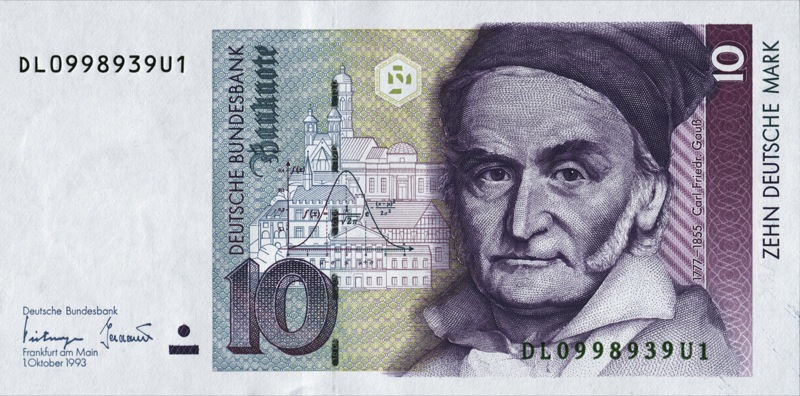
\includegraphics[width=0.618\textwidth]{pictures/gauss}
\caption{10 DM Note: \textsc{Carl Friedrich Gauss}}
\end{center}
\end{figure}
Vor dieser kritischen Revision konnten nur wenige, ausserordentlich f\"ahige Mathematiker mit der Infinitesimalrechnung umgehen, da sie unklar dargestellt wurde und teilweise mit Mystik behaftet war. Man brauchte ein instinktives und sicheres Gef\"uhl f\"ur den richtigen Weg zur L\"osung.
Die Arbeiten der Analytiker des 19. Jahrhunderts haben gezeigt, dass die ganze Infinitesimalrechnung auf nur f\"unf grunds\"atzlichen, klaren mathematischen Ideen beruht:
\begin{itemize}
\item Funktion
\item Behandlung des Krummen via Approximation wie Gerades
\item Konvergenz und Grenzwert
\item Differentiation
\item Integration
\end{itemize}
Dadurch ist heute die Infinitesimalrechnung f\"ur jeden interessierten Menschen zug\"anglich geworden.
Man darf aber nicht den Schluss ziehen, dass die Entwicklung der Analysis im 19. Jahrhundert abgeschlossen worden w\"are. Gegenw\"artig werden in den verschiedenen Teilgebieten der Analysis j\"ahrlich mehr als 1000 Arbeiten ver\"offentlicht.

\subsection{Der Differenzenquotient}
Bei vielen funktionalen Zusammenh\"angen ist nicht nur interessant, welche Werte eine Funktion $f$ annimmt und ob sie stetig ist, sondern auch, wie rasch bzw. stark die Funktionswerte $y=f(x)$ zu- oder abnehmen, wenn sich die $x$-Werte \"andern.

\begin{cdef}[Differenzenquotient]{def:diffquot}
Der \emph{Differenzenquotient}
\marginnote{
\qrcode{
https://www.youtube.com/watch?v=J0FCAuTM9pA}
}
$$\frac{f(x_0+h)-f(x_0)}{h}=\frac{\Delta y}{\Delta x}$$
gibt die durchschnittliche \"Anderung der Funktion $f$ im Intervall $[x_0,x_0+h]$ an.
\end{cdef}

Mit ihm erh\"alt man eine erste grobe Aussage \"uber das \"Anderungsverhalten der Funktion $f$. Dieser Differenzenquotient kann je nach Funktion verschiedene Bedeutungen haben.

\begin{bsp}\label{bspsteigungswinkel}
Bei
\marginnote{
\qrcode{
https://www.youtube.com/watch?v=BOGpb1yyD-E}
}
einer ansteigenden Strasse wird der Differenzenquotient
$$\frac{f(x_0+h)-f(x_0)}{h}=\tan(\alpha)=m.$$
Er entspricht also der durchschnittlichen Steigung des betrachteten Strassenst\"ucks.
\end{bsp}

\begin{ueb}[Könizberg]\label{uebkoenizberg}
Berechne die durchschnittliche Steigung des K\"onizbergs (h\"ochster Punkt 674 M.\"u.M) in Prozent und berechne den Steigungswinkel, wenn die beiden Messungen horizontal $\unit[700]{m}$ auseinander liegen. K\"oniz liegt auf einer H\"ohe von 610 M.\"u.M.
\end{ueb}

\subsubsection{Anwendungen}
\begin{bsp}\label{bspradioaktiv}
Beim radioaktiven Zerfall verringert sich die Anzahl der radioaktiven Kerne allm\"ahlich. Dementsprechend nimmt die Strahlung jedes radioaktiven Pr\"aparats im Laufe der Zeit ab. Die Aktivit\"at sinkt innerhalb der sogenannten \emph{Halbwertszeit} auf die H\"alfte ihres Ausgangswerts. Da radioaktive Materialen aufgrund ihrer ausgesendeten Strahlung leicht geortet werden k\"onnen, dienen radioaktive Isotope in vielen Bereichen der Physik, Chemie, Biologie, Medizin und Technik als Indikatoren. Beispielsweise kann man mit Jod (J-131), das dem Organismus in geringer Menge zugef\"uhrt wird, Stoffwechselvorg\"ange verfolgen und allf\"allige St\"orungen feststellen. Das folgende Diagramm zeigt den Zerfall von J-131, dessen Halbwertszeit 8 Tage betr\"agt.

\begin{figure}
\begin{center}
\definecolor{zzttqq}{rgb}{0.6,0.2,0}
\definecolor{cqcqcq}{rgb}{0.75,0.75,0.75}
\scalebox{0.9}{
\begin{tikzpicture}[line cap=round,line join=round,>=triangle 45,x=0.25cm,y=4.5cm]
\draw [color=cqcqcq,dash pattern=on 3pt off 3pt, xstep=1cm,ystep=1.125cm] (0,0) grid (35,1.1);
\draw[->,color=black] (-4,0) -- (36,0);
\foreach \x in {8,16,24,32}
\draw[shift={(\x,0)},color=black] (0pt,2pt) -- (0pt,-2pt) node[below] {\footnotesize $\x$};
\draw[color=black] (35.04,-0.08) node [anchor=south west] { $t$};
\draw[->,color=black] (0,-0.1) -- (0,1.2);
\foreach \y in {2.5,5,7.5,10}
\draw[shift={(0,0.1*\y)},color=black] (2pt,0pt) -- (-2pt,0pt) node[left] {\footnotesize $\y\cdot10^8$};
\draw[color=black] (0.28,1.15) node [anchor=west] { $N(t)$};
%\draw[color=black] (0pt,-8pt) node[right] {\footnotesize $0$};
\clip(-4,-0.1) rectangle (36,1.2);
\draw[line width=1.2pt,color=zzttqq, smooth,samples=100,domain=0.0:36.0] plot(\x,{1/(2^(\x/8))});
\draw[color=zzttqq] (6.5,0.86) node {Jod$_{131}$};
\end{tikzpicture}
}
\caption{Zerfallsverlauf von Jod 131}\label{jod}
\end{center}
\end{figure}

Der Differenzenquotient
$$\frac{\Delta N(t_0)}{\Delta t}=\frac{N(t_1)-N(t_0)}{t_1-t_0}$$
gibt in diesem Beispiel die durchschnittliche Zerfallsrate des radioaktiven Isotops an.
\end{bsp}

\begin{ueb}[Jod]\label{uebzerfall}
Berechne
\marginnote{
\qrcode{
https://www.youtube.com/watch?v=VgUkjQVWASM}
}
mit Hilfe der Abbildung \ref{jod} auf Seite \pageref{jod} die durchschnittliche Zerfallsrate f\"ur Jod 131 in den Intervallen $[8,16], [16,24]$ und $[5,13]$.
\end{ueb}

\begin{ueb}[Wohnbevölkerung]
In den angewandten Wissenschaften, zum Beispiel National\"okonomie, bezeichnet man den Zuwachs $\Delta y$ einer Ver\"anderlichen $y$ pro Zeitperiode $\Delta t$ als die durchschnittliche Wachstumsrate.
Abbildung \ref{tab:bevoelkerung} auf Seite \pageref{tab:bevoelkerung} zeigt die Wohnbev\"olkerung der Schweiz (in Mio.).
\begin{figure}[h!]
\begin{center}
\definecolor{cqcqcq}{rgb}{0.75,0.75,0.75}
\scalebox{1.85}{
\begin{tikzpicture}[line cap=round,line join=round,>=triangle 45,x=0.6cm,y=0.6cm]
\draw [color=cqcqcq,dash pattern=on 3pt off 3pt, xstep=0.3cm,ystep=0.6cm] (0,0) grid (10.5,7);
\draw[->,color=black] (-1.1,0) -- (10.8,0);
%\foreach \x in {1,2,3,4,5,6,7,8,9,10}
%\draw[shift={(\x,0)},color=black] (0pt,2pt) -- (0pt,-2pt);
\draw[color=black] (10.6,0.1) node [anchor=south west] {$t$};
\draw[->,color=black] (0,-0.55) -- (0,7.2);
\foreach \y in {6.1,6.2,6.3,6.4,6.5,6.6}
\draw[shift={(0,{10*\y-60})},color=black] (2pt,0pt) -- (-2pt,0pt) node[left] {\footnotesize $\y$};
\draw[color=black] (-0.1,7.2) node [anchor=east] {$y$};
\draw[color=black] (-14pt,-18pt) node[right] {\footnotesize $1967$};
\draw[color=black] (19pt,-18pt) node[right] {\footnotesize $70$};
\draw[color=black] (61pt,-18pt) node[right] {\footnotesize $75$};
\draw[color=black] (103pt,-18pt) node[right] {\footnotesize $80$};
\draw[color=black] (145pt,-18pt) node[right] {\footnotesize $85$};
\clip(-1.08,-0.54) rectangle (10.8,7.14);
\draw [line width=1.2pt] (0.5,2.28)-- (0,1.76);
\draw [line width=1.2pt] (0.5,2.28)-- (1,3.4);
\draw [line width=1.2pt] (1,3.4)-- (1.5,3.8);
\draw [line width=1.2pt] (1.5,3.8)-- (2,4.26);
\draw [line width=1.2pt] (2,4.26)-- (3,5.22);
\draw [line width=1.2pt] (3,5.22)-- (3.5,5.34);
\draw [line width=1.2pt] (3.5,5.34)-- (4.5,4.68);
\draw [line width=1.2pt] (4.5,4.68)-- (5,4.46);
\draw [line width=1.2pt] (5,4.46)-- (5.5,4.56);
\draw [line width=1.2pt] (5.5,4.56)-- (6.5,4.44);
\draw [line width=1.2pt] (6.5,4.44)-- (7.02,4.58);
\draw [line width=1.2pt] (7.02,4.58)-- (8,5);
\draw [line width=1.2pt] (8,5)-- (9.5,5.62);
\draw [line width=1.2pt] (9.5,5.62)-- (10,5.7);
\draw [line width=1.2pt] (10,5.7)-- (10.5,6);
\end{tikzpicture}
}
\end{center}
\caption{Wohnbev\"olkerung der Schweiz (in Mio.)}\label{tab:bevoelkerung}
\end{figure}
Berechne die durchschnittliche Wachstumsrate, also den Differenzenquotienten $\frac{\Delta y}{\Delta t}$, der Wohnbev\"olkerung der Schweiz in den Zeitperioden 1968-1972, 1972-1975 und 1977-1980.
\end{ueb}

\begin{ueb}[Differenzenquotient]\label{uebdifferenzenquotient}
Berechne die durchschnittliche Steigung des Graphen der Funktion $f$ im Intervall $[x_0,x_0+h]$, und best\"atige dein Ergebnis mit einer Skizze.
\begin{enumeratea}
\item $f(x)=x^2$ in $[1,1.2]$
\item $f(x)=\sin(x)$ in $[0,\pi/2]$
\item $f(x)=\ln(x)$ in $[0.5,e]$
\item $f(x)=e^{x/2}$ in $[-1,1]$
\item In welchem Intervall $[2,b]$ betr\"agt die durchschnittliche Steigung der Funktion aus (a) $6$?
\end{enumeratea}
\end{ueb}

\begin{ueb}[Computer]\label{uebcomputer}
Eine neue Computeranlage f\"ur ein gr\"osseres Unternehmen kostet $\unit[500\,000]{CHF}$. Ihr Wert nach $t$ Jahren betr\"agt etwa
$$W(t)=500\,000\cdot e^{-0.35t}.$$
Berechne ihre durchschnittliche Wert\"anderung pro Jahr zwischen dem 2. und 5. Jahr.
\end{ueb}

Abschliessend zur Anwendung des Differenzenquotienten noch aus der Chemie folgendes
\begin{bsp}
Bei chemischen Reaktionen gibt es keine einfache Methode, um die Reaktionsrate, d.h. die Geschwindigkeit, mit der die Reaktion abl\"auft, direkt zu messen. \"Ublicherweise misst man die Konzentration des Ausgangsmaterials oder des Endprodukts zu verschiedenen Zeitpunkten und liest dann aus einer graphischen Darstellung die Reaktionsrate zu einem bestimmten Zeitpunkt ab.
\end{bsp}

\section{Der Differenzialquotient}
\subsection{Von der mittleren zur momentanen \"Anderungsrate}
\begin{wrapfigure}{r}{0.382\textwidth}
  \begin{center}
    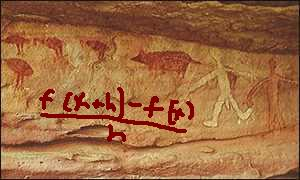
\includegraphics[width=0.382\textwidth]{pictures/cave}
  \end{center}
%\caption{You Know my Name}
\end{wrapfigure}
In fr\"uheren Aufgaben wurde die durchschnittliche \"Anderung einer Gr\"osse berechnet; beispielsweise die durchschnittliche Geschwindigkeit einer Rakete, wenn man das Weg-Zeit-Diagramm kennt:
$$\bar{v}=\frac{\Delta s}{\Delta t}$$
wobei $\Delta s$ die H\"ohendifferenz und $\Delta t$ die L\"ange des zugeh\"origen Zeitintervalls ist.
Wie gross ist aber die Geschwindigkeit zu einem bestimmten Zeitpunkt, zum Beispiel $\unit[15]{s}$ nach dem Start? Einen ersten, noch ungenauen N\"aherungswert f\"ur die gesuchte Momentangeschwindigkeit liefert sicher die mittlere Geschwindigkeit im Zeitintervall $[15,20]$. Durch die Verkleinerung des Zeitintervalls kann die Genauigkeit verbessert werden (siehe \"Ubung 1, \"Ubungen zum Differenzenquotienten). Die entsprechende mathematische Formulierung lautet:
Die Momentangeschwindigkeit $v(t_0)$ zum Zeitpunkt $t_0$ ist der Grenzwert, gegen den die Durchschnittsgeschwindigkeit $\bar{v}$ im Zeitintervall $\Delta t=t_1-t_0$ strebt, wenn $t_1$ gegen $t_0$ geht ($\Delta t\rightarrow 0$). In Formeln:
$$v(t_0)=\lim_{t_1\rightarrow t_0}\bar{v}=\lim_{t_1\rightarrow t_0}\frac{\gD s}{\gD t}=\lim_{t_1\rightarrow t_0}\frac{s(t_1)-s(t_0)}{t_1-t_0}.$$
$s(t)$ bezeichne  die bis zum Zeitpunkt $t$ erreichte H\"ohe.

\begin{ueb}[freier Fall]\label{uebfreierfall}
F\"allt ein K\"orper aus der Ruhelage im freien Fall $t$ Sekunden lang, so l\"asst sich der zur\"uckgelegte Weg $s$ (in Meter) ann\"ahernd durch
$$s(t)=5t^2$$
berechnen.

Berechne die Durchschnittsgeschwindigkeiten in den Zeitintervallen $[3,3.5]$, $[3,3.2]$, $[3,3.1]$, $[3,3.05]$. Wie gross ist die Momentangeschwindigkeit nach genau drei Sekunden?
\end{ueb}

\subsection{Das Konzept}
Eine beliebige Funktion $f$ sei im betrachteten Intervall $[a,b]$ stetig. Mit der Steigung der Sekante l\"asst sich das \"Anderungsverhalten der Funktion, d.h. die Steigung, an einer beliebigen, aber festgehaltenen Stelle $x_0\in[a,b]$ in einfacher Weise erkl\"aren. Will man nun das \"Anderungsverhalten der Funktion in $x_0$ exakt bestimmen, so ist dazu die Tangentensteigung im Punkt $P=\point{x_0}{f(x_0)}$ zu berechnen.

\begin{figure}
\begin{center}
\definecolor{ffqqtt}{rgb}{1,0,0.2}
\definecolor{xdxdff}{rgb}{0.5,0.5,1}
\definecolor{uququq}{rgb}{0.25,0.25,0.25}
\scalebox{0.85}{
\begin{tikzpicture}[line cap=round,line join=round,>=triangle 45,x=0.35cm,y=1cm]
\draw[->,color=uququq] (-2.53,0) -- (18.47,0);
\foreach \x in {-2,2,4,6,8,10,12,14,16,18}
\draw[shift={(\x,0)},color=uququq] (0pt,-2pt);
\draw[color=uququq] (17.99,0.05) node [anchor=south west] {$x$};
\draw[->,color=uququq] (0,-0.69) -- (0,5.12);
\foreach \y in {,1,2,3,4,5}
\draw[shift={(0,\y)},color=uququq] (2pt,0pt) -- (-2pt,0pt);
\draw[color=uququq] (0.14,4.87) node [anchor=west] {$y$};
\clip(-2.53,-0.69) rectangle (18.47,5.12);
\draw[line width=1pt, smooth,samples=100,domain=-2.53:18.48] plot(\x,{0.02*\x^2+0.5});
\draw [domain=-2.53:18.47] plot(\x,{(-0.72--3.84*\x)/12});
\draw [domain=-2.53:18.47] plot(\x,{(--0.54--2.34*\x)/9});
\draw [domain=-2.53:18.47] plot(\x,{(--1.08--1.2*\x)/5.99});
\draw [dash pattern=on 4pt off 4pt] (14,4.42)-- (13.92,0);
\draw [dash pattern=on 4pt off 4pt] (2,0.58)-- (13.93,0.67);
\draw [dash pattern=on 4pt off 4pt] (2,0.58)-- (2,0);
\draw [line width=1pt,color=ffqqtt,domain=-2.53:18.47] plot(\x,{(--0.42--0.08*\x)/1});
\draw [color=ffqqtt](11.52,1.86) node[anchor=north west] {$t$};
\draw (7.53,0.63) node[anchor=north west] {$\Delta x$};
\draw (14.4,2.72) node[anchor=north west] {$\Delta f$};
\draw (12.8,4.86) node[anchor=north west] {$Q$};
\draw (1.5,-0.1) node[anchor=north west] {$x_0$};
\draw (13.2,-0.1) node[anchor=north west] {$x$};
\draw[color=black] (-1.9,0.85) node {$f$};
\fill [color=black] (2,0.58) circle (1.5pt);
\draw[color=black] (1.74,0.82) node {$P$};
\fill [color=xdxdff] (14,4.42) circle (1.5pt);
\fill [color=xdxdff] (11,2.92) circle (1.5pt);
\fill [color=xdxdff] (7.99,1.78) circle (1.5pt);
\end{tikzpicture}
}
\caption{\"Ubergang vom Differenzenquotienten zum Differenzialquotient}
\end{center}
\end{figure}

\pagebreak

\begin{cdef}[Steigung]{def:steigung}
Die Steigung der Tangente in $P$ wird als \emph{Steigung} des Graphen in $P$, also als momentanes \"Anderungsverhalten der Funktion $f$ an einer Stelle $x_0$ bezeichnet.
\end{cdef}

Nachdem die Tangente im Punkt eines Graphen definiert ist, kann das Tangentenproblem rechnerisch formuliert werden. Es gen\"ugt, die Steigung der Tangente in $P$ zu ermitteln, da die Stelle $x_0$ bzw. der Punkt $P$ gegeben ist, womit die Lage der Tangente eindeutig bestimmt ist.

\begin{cdef}[Differenzialquotient]{def:difftquot}
Die Steigung der Tangente erh\"alt man f\"ur $\gD x\rightarrow0$. Sie ist also
$$\lim_{x\rightarrow x_0}\frac{\gD f(x_0)}{\gD x}=\lim_{x\rightarrow x_0}\frac{f(x)-f(x_0)}{x-x_0}.$$
Falls dieser Grenzwert existiert, was ja keinesfalls sicher ist, da sowohl der Z\"ahler als auch der Nenner gegen Null streben ($x_0$ ist eine Unbestimmtheitsstelle), nennt man diesen Grenzwert den \emph{Differenzialquotient} von $f$ an der Stelle $x_0$.
\end{cdef}

Der Differenzialquotient ist der wichtigste Begriff der Differenzialrechnung. Mit ihm bew\"altigten Newton und Leibniz den \"Ubergang von der antiken zur modernen Mathematik, da sie jetzt das momentane \"Anderungsverhalten einer Funktion bzw. die Steigung des Graphen an einer bestimmten Stelle $x_0$ rechnerisch untersuchen konnten.
Sowohl der Name \emph{Differenzialquotient} als auch die Schreibweise $\frac{\mathrm{d}f(x_0)}{\mathrm{d}x}$ stammen von \textsc{Leibniz}.

F\"ur die praktische Berechnung des Differenzialquotienten ersetzt man $x$ durch $x_0+h$ und l\"asst $h$ gegen $0$ streben. Der Differenzialquotient erh\"alt dann die Form
$$\frac{\mathrm{d}f(x_0)}{\mathrm{d}x}=\lim_{h\rightarrow0}\frac{f(x_0+h)-f(x_0)}{h}.$$

\begin{ueb}[\"Anderungsraten]
Vervollst\"andige Tabelle \ref{tab:interpretation} auf Seite \pageref{tab:interpretation} mit weiteren Beispielen f\"ur lokale \"Anderungsraten.

\begin{table}
\large
\begin{center}
\begin{tabular}{|c|c|c|}
\hline
\spaltenheight $x$ & $f(x)$ & $\frac{\mathrm{d}f(x)}{\mathrm{d}x}$ \spaltensep\hline
\spaltenheight Abszisse & Ordinate & Graphensteigung \spaltensep\hline
\spaltenheight Zeit & Ort & \spaltensep\hline
\spaltenheight Zeit & & Beschleunigung \spaltensep\hline
\spaltenheight Zeit & elektrische Ladung & \spaltensep\hline
\spaltenheight  & Energie & Leistung \spaltensep\hline
\spaltenheight  & chem. Konzentration & chem. Reaktionsgeschw.\spaltensep\hline
\spaltenheight  Zeit & & Wachstumsgeschwindigkeit \spaltensep\hline
\spaltenheight  Zeit & Geldwert & \spaltensep\hline
\end{tabular}
\end{center}
\caption{Interpretation des Differenzialquotienten}\label{tab:interpretation}
\end{table}
\end{ueb}

\begin{ueb}[Differenzialquotient]\label{uebtangente}
Berechne
\marginnote{
\qrcode{
https://www.youtube.com/watch?v=z-42d5dtA_Q}
}
den Differenzialquotienten der Funktion $f$ an der Stelle $x_0$ und die Gleichung der Tangente im Punkt $P\point{x_0}{f(x_0)}$. \"Uberpr\"ufe Ihr Ergebnis mit einer Skizze.
\begin{enumeratea}
\item $f(x)=x^2$ in $x_0=1$
\item $g(x)=-x^3$ in $x_0=-1$
\item $h(x)=x^{-1}$ in $x_0=0.25$
\end{enumeratea}
\end{ueb}

\begin{ueb}[Momentangeschwindigkeit]\label{uebmomentangeschw}
Berechne
\marginnote{
\qrcode{
https://www.youtube.com/watch?v=-KFROqbQkuA}
}
die Momentangeschwindigkeit zur Zeit $t=2$ f\"ur eine Bewegung mit

\begin{minipage}{3.5cm}
\begin{enumeratea}
\item $s(t)=t^2+3t$
\end{enumeratea}
\end{minipage}
\begin{minipage}{3.5cm}
\begin{enumeratea}
\addtocounter{enumi}{1}
\item $s(t)=\sqrt{t}$
\end{enumeratea}
\end{minipage}

wenn $t$ in Sekunden und $s(t)$ in Meter angegeben sind.
\end{ueb}

\section{Die Ableitung}
\subsection{Definition}

\begin{cdef}[Ableitung]{def:ableitung}
Existiert f\"ur jedes $x$ in einem Intervall der Grenzwert
$$\lim_{h\to0}\frac{f(x+h)-f(x)}{h}=\frac{\mathrm{d}f(x)}{\mathrm{d}x}$$
so kann damit eine neue Funktion $f'$ definiert werden. Bei dieser Funktion $f'$ wird jedem $x$ aus dem Intervall genau eine reelle Zahl, n\"amlich $\frac{\mathrm{d}f(x)}{\mathrm{d}x}$, zugeordnet.

Diese Funktion $f'$ --- die Symbolik stammt \"ubrigens von Leonard Euler --- nennt man Steigungsfunktion, weil jedem $x$ eine Steigung zugeordnet wird. Durch $f'$ wird das \"Anderungsverhalten der Ausgangsfunktion $f$ charakterisiert. $f'$ wird oft kurz als \emph{Ableitung} von $f$ bezeichnet.
\end{cdef}

\begin{ueb}[Steigungsfunktion]\label{uebsteigungsfunktion}
Ermittle
\marginnote{
\qrcode{
https://www.youtube.com/watch?v=5RJYwSTO5w8}
}
die Steigungsfunktion (die Ableitung) $f'$ f\"ur
\begin{enumeratea}
\item die Geraden mit den Gleichungen $f(x)=x$, $f(x)=2x-3$,
\item die Parabeln mit den Gleichungen $f(x)=x^2$, $f(x)=3x^2-2$,
\item die Hyperbeln mit der Gleichung $f(x)=\frac{2}{x}$
\item den Parabelast mit der Gleichung $f(x)=\sqrt{x}$,
\end{enumeratea}
und die Steigungen in den Punkten $P\point{3}{?}$ und $Q\point{-2}{?}$.
\end{ueb}

\begin{ueb}[\glqq Potenzregel\grqq]\label{uebtabelle}
Vervollst\"andige
\marginnote{
\qrcode{
https://www.youtube.com/watch?v=O722WzomYN4}
}
die Tabelle \ref{tab:abl} auf Seite \pageref{tab:abl}.

\begin{table}
\Huge
\begin{center}
\begin{tabular}{|c|c|}
\hline
\rule[-5mm]{0pt}{13mm}$f(x)=$ & $f'(x)=$\\ \hline
\rule[-5mm]{0pt}{15mm}$x^4$ & \\ \hline
\rule[-5mm]{0pt}{15mm}$x^3$ & \\ \hline
\rule[-5mm]{0pt}{15mm}$x^2$ & \\ \hline
\rule[-5mm]{0pt}{15mm}$x$ & \\ \hline
\rule[-5mm]{0pt}{15mm}$x^0$ & \\ \hline
\rule[-5mm]{0pt}{15mm}$\frac{1}{x}=x^{-1}$ & \\ \hline
\rule[-6mm]{0pt}{16mm}$\frac{1}{x^2}=x^{-2}$ & \\ \hline
\rule[-5mm]{0pt}{17mm}$\sqrt{x}=x^{\frac{1}{2}}$ & \\ \hline
\rule[-5mm]{0pt}{17mm}$\sqrt[3]{x}=x^{\frac{1}{3}}$ & \\ \hline
\rule[-5mm]{0pt}{17mm}$\sqrt{x^3}=x^{\frac{3}{2}}$ & \\ \hline
\end{tabular}
\caption{Wichtige Ableitungen}\label{tab:abl}
\end{center}
\end{table}
\end{ueb}

\subsection{Ableitungsregeln}

Die
\marginnote{
\qrcode{
https://www.youtube.com/watch?v=Jv0QEd45vqY}
}
vorherigen Aufgaben waren teilweise Beispiele f\"ur die folgenden allgemeinen Differenziations\-regeln. Die beiden Funktionen $f$ und $g$ seien im betrachteten Intervall differenzierbar. Dann gelten:

\begin{itemize}
\item Eine konstante Funktion hat die Ableitung $0$.
$$(c)'=0$$
\item Ein konstanter Summand f\"allt bei der Differenziation weg.
$$(f(x)+c)'= f'(x)$$
\item Ein konstanter Faktor bleibt bei der Differenziation erhalten.
$$(cf(x))'=cf'(x)$$
\item Eine Summe von Funktionen darf man gliedweise differenzieren.
$$(f(x)+g(x))'=f'(x)+g'(x)$$
\end{itemize}

\begin{ueb}[Ableitungsregeln]\label{uebbeweis}
Beweise die vier Regeln mittels
$$F'(x)=\lim_{h\to0}\frac{F(x+h)-F(x)}{h}$$
\end{ueb}

\begin{ueb}[üben]\label{uebdifferenzieren}
Differenziere die Funktionen

\begin{minipage}{5cm}
\begin{enumeratea}
\item $\frac{1}{2}x^2-3x+2$
\item $5x^3+\frac{1}{3}x^2-2x-7$
\end{enumeratea}
\end{minipage}
\begin{minipage}{5cm}
\begin{enumeratea}
\addtocounter{enumi}{2}
\item $\frac{2}{x}-3x$
\item $\sqrt{x}-10x-(4x)^2$
\end{enumeratea}
\end{minipage}
\end{ueb}

\begin{ueb}[Glukose]\label{uebglukose}
F\"ur
\marginnote{
\qrcode{
https://www.youtube.com/watch?v=CYY4jeCU_z4}
}
die Masse $M$ (in g) von Glukose bei einem Stoffwechselexperiment in Abh\"angigkeit der Zeit $t$ (in h) gilt:
$$M(t)=4.5-0.03t^2.$$
\begin{enumeratea}
\item Wie gross ist die durchschnittliche \"Anderungsrate in den ersten beiden Stunden?
\item Berechne die momentane \"Anderungsrate f\"ur $t=0$ und $t=2$.
\end{enumeratea}
\end{ueb}

\begin{ueb}[Kugel]\label{uebvolumen}
Differenziere die Funktion $V$, deren Funktionswerte das Volumen einer Kugel mit dem Radius $r$ angeben. Was f\"allt auf?
\end{ueb}

\begin{ueb}[Hängebrücke]\label{uebbrucke}
Die
\marginnote{
\qrcode{
https://www.youtube.com/watch?v=4nFIPeEDeMQ}
}
Tragseile einer H\"angebr\"ucke sind an den Pfeilern befestigt, die $\unit[250]{m}$ auseinander stehen, und h\"angen in Form einer Parabel, deren tiefster Punkt $\unit[50]{m}$ unter den Aufh\"angungspunkten liegt. Ermittle den Winkel zwischen Seil und Pfeiler.
\end{ueb}

\begin{ueb}[Was wäre München ohne da Wisn?]
Am
\marginnote{
\qrcode{
https://www.youtube.com/watch?v=Qsh0g0nuaoo}
}
Oktoberfest in M\"unchen sind in einem grossen Fass Bier anf\"anglich $\unit[2000]{Liter}$ Bier. Der Inhalt $V(t)$ des Fasses l\"asst sich in Abh\"angigkeit der Zeit $t$ in Minuten durch
$$V(t)=2000-\frac{5}{48}t^2+\frac{1}{3456}t^3$$
beschreiben.
\begin{enumeratea}
\item Zeige, dass das Fass nach vier Stunden leer ist.
\item Wie viel Liter Bier fliessen genau 30 Minuten nach dem Anstich des Fasses in die Humpen?
\item Wann ist das Fest auf seinem \glqq H\"ohepunkt\grqq?
\end{enumeratea}
\end{ueb}

\begin{ueb}[Wildsaison]
The
number of deer in a forest $t$ years after beginning of a population study is shown by the graph in figure \ref{deer} on page \pageref{deer}.

\begin{figure}
\begin{center}
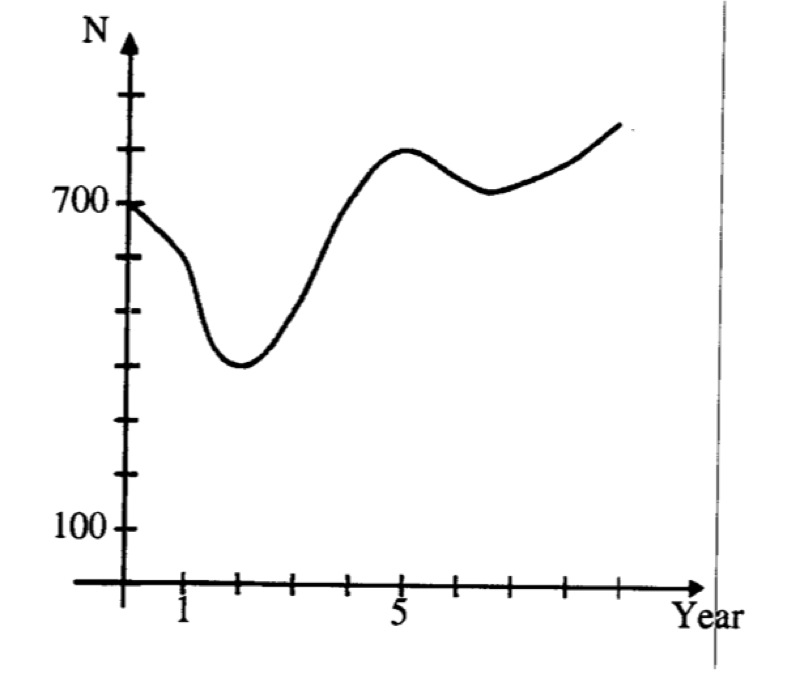
\includegraphics[width=0.55\textwidth,angle=0.8]{pictures/deer}
\end{center}
\caption{Wildbestand \"uber 10 Jahre}\label{deer}
\end{figure}

\begin{enumeratea}
\item Over which of the following time intervals did the population of deer decline at an average rate of 50 deer per year? [0, 1], [1,2], [1,3], [1,4], [5,6]
\item When was the population of deer increasing most rapidly?
\item Approximately how fast was the population of deer increasing or decreasing 1.5 years after the study began?
\end{enumeratea}
\end{ueb}

\begin{ueb}[match]
Finde
\marginnote{
\qrcode{
https://www.youtube.com/watch?v=ZITSx3cx0L0}
}
zu den fünf Graphen a -- e in Abbildung \ref{derive} auf Seite \pageref{derive} jeweils die passende Ableitungsfunktion A -- E.

\begin{figure}
\begin{center}
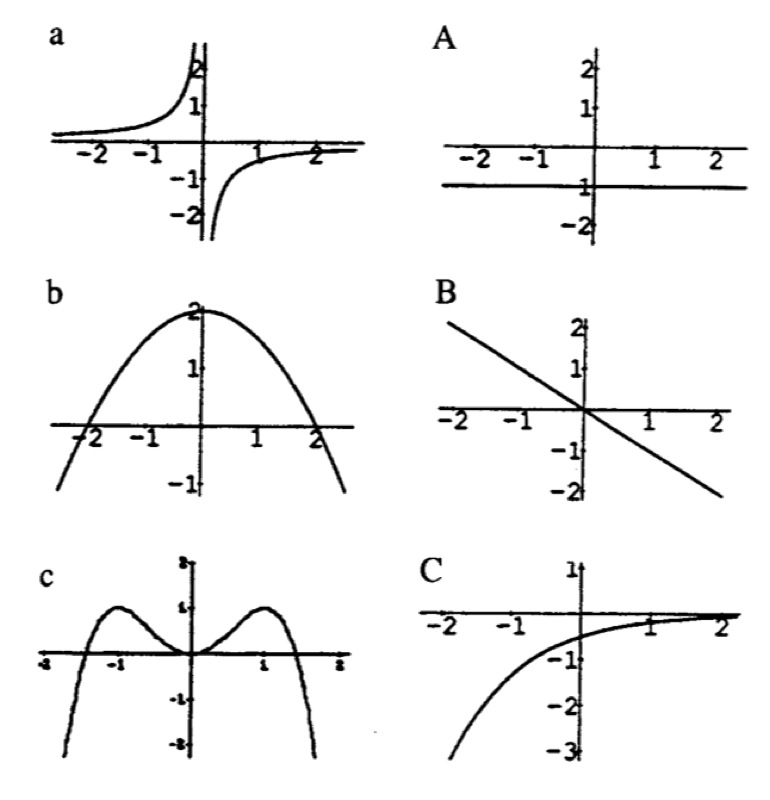
\includegraphics[width=0.45\textwidth,angle=0.6]{pictures/derivates1}
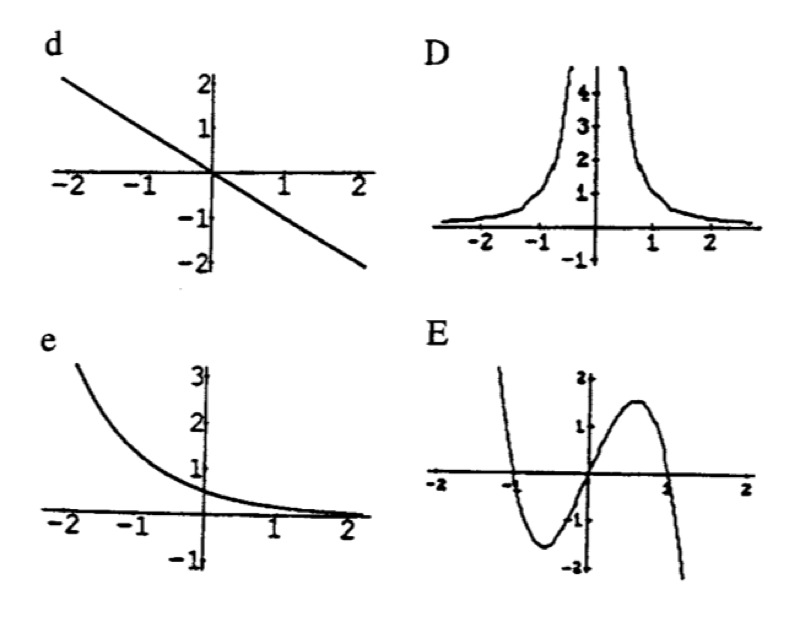
\includegraphics[width=0.45\textwidth,angle=0.6]{pictures/derivates2}
\end{center}
\caption{Graphen und ihre Ableitungsgraphen}\label{derive}
\end{figure}
\end{ueb}

\section{Weitere Ableitungsregeln}
Wollte man die Ableitung der Funktion
$$f(x)=\sin^3(x)\quad\text{oder}\quad g(x)=\frac{3x^2-7x+1}{x^3-2}$$
mittels dem Differenzialquotienten
$$\lim_{h\to0}\frac{f(x+h)-f(x)}{h}$$
berechnen, so w\"are dies sicher ein m\"uhsames Unterfangen. Mit einigen weiteren Differenziationsregeln lassen sich die n\"otigen Rechnungen erheblich vereinfachen.
\subsection{Produkt- und Quotientenregel}
Aus
$$f(x)=x^5=x^2\cdot x^3$$
und daraus
$$f'(x)=5x^4\neq 2x\cdot3x^2$$
erkennt man, dass die Ableitung eines Produkts nicht so einfach wie bei der Summe berechnet werden kann. Sowohl f\"ur das Produkt als auch den Quotienten von Funktionen bedarf es einer besonderen Regel.

\begin{csatz}[Die Produktregel]{satz:prodregel}
Sind
\marginnote{
\qrcode{
https://www.youtube.com/watch?v=KsMlJTZOaLA}
}
$f$ und $g$ an der Stelle $x$ differenzierbar, so ist auch ihr Produkt an dieser Stelle differenzierbar. Der Differenzialquotient von $F(x)=f(x)\cdot g(x)$ lautet:
$$F'(x)=f'(x)\cdot g(x)+f(x)\cdot g'(x).$$
\end{csatz}
\begin{csatz}[Die Reziprokregel]{satz:rezi}
Ist
\marginnote{
\qrcode{
https://www.youtube.com/watch?v=ENdiTNVNVMw}
}
$g$ an der Stelle $x$ differenzierbar und $g(x)­0$, so ist auch $1/g$ an dieser Stelle differenzierbar. Der Differenzialquotient von $F(x)=1/g(x)$ lautet:
$$F'(x)=-\frac{g'(x)}{g(x)^2}.$$
\end{csatz}
\begin{csatz}[Die Quotientenregel]{satz:quot}
Sind $f$ und $g$ an der Stelle $x$ differenzierbar und $g(x)­0$, so ist auch ihr Quotient $f/g$ an dieser Stelle differenzierbar. Der Differenzialquotient von $F(x)=f(x)/g(x)$ lautet:
$$F'(x)=\frac{f'(x)g(x)-f(x)g'(x)}{g(x)^2}.$$
\end{csatz}
\begin{proof}[Beweis der Produktregel]
\begin{align*}
F'(x)&=\lim_{h\to0}\frac{F(x+h)-F(x)}{h}=\\
&=\lim_{h\to0}\frac{f(x+h)g(x+h)-f(x)g(x)}{h}=\\
&=\lim_{h\to0}f(x+h)\frac{g(x+h)-g(x)}{h}+\\
&\q+\lim_{h\to0}\frac{f(x+h)-f(x)}{h}g(x)
\end{align*}
Da $f$ an der Stelle $x$ nach Voraussetzung differenzierbar ist, also dort sicher auch stetig, gilt $\lim_{h\to0}f(x+h)=f(x)$. Und daraus erh\"alt man bereits:
$$F'(x)=f(x)\cdot g'(x)+f'(x)\cdot g(x)$$
\end{proof}

\begin{ueb}[Quotientenregel]\label{uebquotientenregel}
Beweise die Quotientenregel indem du
$$F(x)=\frac{f(x)}{g(x)}=f(x)\cdot\frac{1}{g(x)}$$
setzt und die Produktregel benutzt.
\end{ueb}
\begin{ueb}[ueb ueb]\label{uebableitungen}
Ermittle die Definitionsmenge und die Ableitung der folgenden Funktionen:

\begin{minipage}{9cm}
\begin{enumeratea}
\item $f(x)=(x^2-1)(x^3+4)$
\item $f(x)=(x^3-2x+1)(2x^5+x^4-3x)$
\item $f(x)=\frac{x^4}{4}+3x^3+\frac{x^2}{2}+5x^{-3}$
\item $f(t)=(1+\frac{1}{t})(1-\frac{1}{t^2})$
\item $f(x)=\sqrt{7x}-5x+3x^{-1}+\frac{1}{8}x^8+\frac{1}{5}x^{-5}$
\item $f(t)=\frac{1}{t^2-1}$
\item $f(s)=\frac{4+s}{4-s}$
\end{enumeratea}
\end{minipage}
\begin{minipage}{6cm}
\begin{enumeratea}
\addtocounter{enumi}{7}
\item $f(x)=\frac{2x^2+1}{x+3}$
\item $f(t)=\frac{2t}{1+t^2}$
\item $f(x)=\frac{x^2-1}{x^2-4}$
\item $f(x)=\frac{x-5}{x^2-7x+12}$
\item $f(u)=\frac{u+1}{\sqrt{u}}$
\item $f(t)=\frac{1+\sqrt{t}}{1-\sqrt{t}}$
\end{enumeratea}
\end{minipage}
\end{ueb}
\begin{ueb}[Tangente]\label{uebtangenten}
Berechne im Punkt $P\point{3}{?}$ die Gleichung der Tangente an den Graphen der Funktion
$$f(x)=\frac{1-x}{1+x}.$$
In welchem Punkt hat der Graph eine zur ersten Winkelhalbierenden $g(x)=x$ parallele Tangente?
\end{ueb}

\subsection{Verkettung von Funktionen}
Die wichtigste Regel f\"ur die Differenziation bezieht sich auf zusammengesetzte Funktionen:
$$F(x)=g(f(x)),$$
oder auch etwa in der Form
$$F(x)=g(u)\q\text{mit}\q u=f(x)$$
notiert. Zusammengesetzte Funktionen werden auch \emph{verkettete Funktionen} genannt.
\begin{bsp}
Die Funktion
$$F(x)=\sin(3x)$$
kann als Verkettung mit
$$g(u)=\sin(u)\q\text{und}\q f(x)=3x$$
interpretiert werden.
\end{bsp}
\begin{figure}[b]
\begin{center}
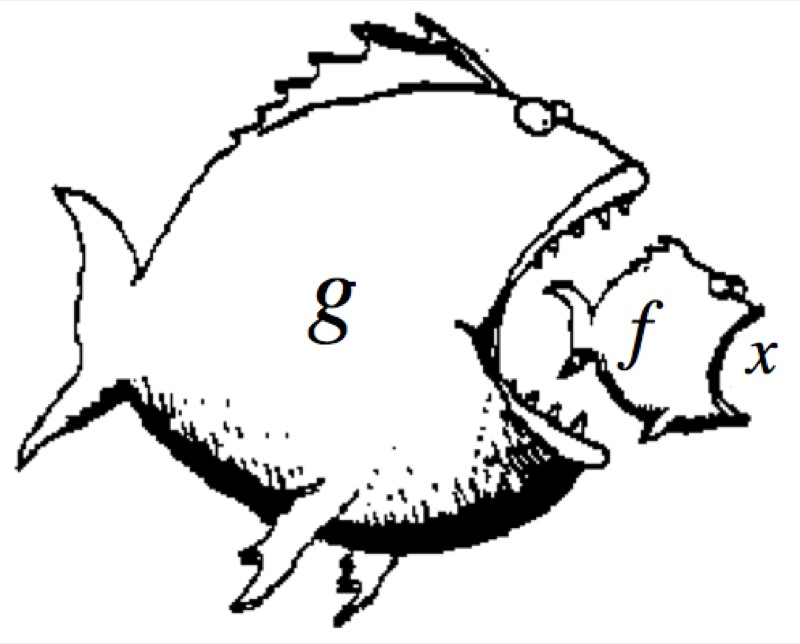
\includegraphics[width=0.15\textwidth]{pictures/verkettung}
\end{center}
\caption{Verkettung von Funktionen: hier $g(f(x))$}
\end{figure}
In der Mathematik ist die Schreibweise
$$(g\circ f)(x)=g(f(x))\q\text{(sprich: g Ring f)}$$
\"ublich; insbesondere dann, wenn die Funktionen ohne Argument notiert werden. Beachten Sie, dass $g\circ f$ bedeutet, dass zuerst $f$ und dann $g$ ausgef\"uhrt wird. Die Reihenfolge ist also von rechts nach links zu lesen.

\begin{ueb}[Ring]\label{uebring}
Ermittle die aus $f$ und $g$ zusammengesetzte Funktion
$$F=g\circ f$$
mit dem Funktionsterm $F(x)=g(f(x))$ und kontrolliere dein Ergebnis mit $x=a$.
\begin{enumeratea}
\item $f(x)=2x-1$, $g(x)=(x-3)^2+5$, $x=3$.
\item $f(x)=x^2+1$, $g(x)=x^3+x^{-2}$, $x=1$.
\end{enumeratea}
\end{ueb}

\subsection{Die Kettenregel}
\begin{csatz}[Die Kettenregel]{satz:chain}
\marginnote{
\qrcode{
https://www.youtube.com/watch?v=ZGOirKbLJUU}
}
$f$ an der Stelle $x$ und $g$ an der Stelle $f(x)$ differenzierbar, so ist auch ihre Verkettung $F=g\circ f$ mit $F(x)=g(f(x))$ in $x$ differenzierbar. Der Differenzialquotient von $F(x)=g(f(x))$ lautet:
$$F'(x)=g'(f(x))\cdot f'(x).$$
\end{csatz}
\begin{bem}
Man nennt $g$ die \"aussere, $f$ die innere Funktion und entsprechend $g'(f(x))$ die \"aussere und $f'(x)$ die innere Ableitung.
\end{bem}
\begin{bsps}
F\"ur $F(x)=(10x^2-7x+3)^{100}$ ist $g(u)=u^{100}$ und $f(x)=10x^2-7x+3$, also $$F'(x)=100(10x^2-7x+3)^{99}\cdot(20x-7).$$

F\"ur $f(x)=\sqrt{5x^7+3x^2+256}$ ist $g(u)=\sqrt{u}$ und $h(x)=5x^7+3x^2+256$, damit $$f'(x)=\frac{35x^6+6x}{2\sqrt{5x^7+3x^2+256}}.$$
\end{bsps}

\begin{proof}[Beweis der Kettenregel]
Es sei $u=f(x)$, $f(x+h)=f(x)+h*$, $h*­0$. Aus der Stetigkeit von $f$ folgt: f\"ur $h\to0$ gilt auch $h*\to0$. So ergibt sich
\begin{align*}
F'(x)&=\lim_{h\to0}\frac{g(f(x+h))-g(f(x))}{h}=\\
&=\lim_{h\to0}\frac{g(u+h*)-g(u)}{h*}\cdot\frac{h*}{h}\\
&=\lim_{h\to0}\frac{g(u+h*)-g(u)}{h*}\cdot\frac{f(x+h)-f(x)}{h}\\
&=g'(u)\cdot f'(x).
\end{align*}
\begin{bem}
Dieser Beweis f\"ur die Kettenregel ist nur f\"ur Funktionen valid, f\"ur die $f(x+h)\to f(x)$ für $h\to 0$. Diese Bedingung ist im allgemeinen erf\"ullt; jedoch beispielsweise f\"ur konstante Funktionen nicht, die aber wegen $(c)'=0$ nicht die Anwendung der Kettenregel erfordern.
\end{bem}
\end{proof}

\begin{ueb}[ueb ueb ueb]\label{uebkettenregel}
Ermittle die Ableitung der Funktionen:

\begin{minipage}{0.45\textwidth}
\begin{enumerate}[a)]
    \item $f(x)=(4x^3-2x)^5$
    \item $f(x)=(x^2+x^{-1})^4$
    \item $f(x)=(x^2-5x+6)^{-3}$
\end{enumerate}
\end{minipage}
\begin{minipage}{0.45\textwidth}
\begin{enumeratea}
\setcounter{enumi}{3}
\item $f(t)=\sqrt{1+t^2}$
\item $f(t)=\left(\frac{t^2+1}{t^2-1}\right)^2$
\item $f(u)=\frac{1}{\sqrt{25-u^2}}$
\end{enumeratea}
\end{minipage}
\end{ueb}

\begin{ueb}[Kläranlage]\label{uebklaranlage}
Wegen eines Defektes musste die Kl\"aranlage eines Dorfes f\"ur einige Stunden abgestellt werden. Die Abwasser wurden in dieser Zeit ungekl\"art in den nahen See geleitet. $f(t)$ sei ein Mass f\"ur die Sauerstoffmenge, die sich $t$ Tage nach dem Zwischenfall im Seewasser befindet. Wasserproben ergaben
$$f(t)=500\left(1-\frac{10}{t+10}+\frac{100}{(t+10)^2}\right).$$
Wie \"andert sich die Sauerstoffmenge am 5. bzw. am 15. Tag nach dem Vorfall?
\end{ueb}

\begin{ueb}[Vochi]\label{uebvoci}
\textsc{L.L.Thurston} entwickelte 1930 eine Formel f\"ur die Berechnung der Zeiteinheiten $T$, die man braucht, um $n$ Dinge (z.B. Vokabeln) auswendig zu lernen:
$$T(n)=\frac{c}{k}n\sqrt{n-a},$$
wobei $a,c,k$ empirisch ermittelte Konstanten sind.

Berechne f\"ur den Fall $a=c=2, k=30$, wobei $T$ die Einheit Minuten hat,
\begin{enumeratea}
\item $T(60)$ und $T(120)$,
\item $T'(11)$ und $T'(27)$.
\end{enumeratea}
\end{ueb}
\begin{ueb}[Calcium]\label{uebcalcium}
Einem Patienten wird eine kleine Menge radioaktives Calcium in die Blutbahn gespritzt. W\"ahrend einigen Tagen wird das verbliebene Calcium im Blut gemessen mit dem Ergebnis, dass nach $t$ Tagen noch
$$C(t)=\unitfrac[0.5(2t+1)^{-0.5}]{mg}{cm^3}$$
vorhanden sind. Berechne die lokale \"Anderungsrate nach a) $0$, b) $4$, c) $7.5$ Tagen.
\end{ueb}

\subsection{Ableitung der trigonometrischen Funktionen}
\begin{ueb}[Trigoableitungen]
Vermute
\marginnote{
\qrcode{
https://www.youtube.com/watch?v=2pExH_iwS9I}
}
aufgrund einer Zeichnung, welche Gestalt die Steigungsfunktion der Sinusfunktion hat.
\end{ueb}

\begin{ueb}[diff tan]
Leite
\marginnote{
\qrcode{
https://www.youtube.com/watch?v=BH7eAN73sYM}
}
die Ableitungsfunktion von
$$f(x)=\tan(x)$$
her.
\end{ueb}

\clearpage

\begin{ueb}[ueb macht Meister]
Bestimme die Ableitung:

\begin{minipage}{0.4\textwidth}
\begin{enumeratea}
\item $f(x)=\sin x+2\cos x$
\item $f(x)=x\sin x+\cos x$
\item $f(x)=\frac{1}{1+\cos x}$
\item $f(u)=\tan^2u$
\item $f(t)=\frac{t^2}{\sin t}$
\item $f(\varphi)=\frac{1}{2}a^2\sin\varphi$
\item $f(x)=\sin(4x)$
\end{enumeratea}
\end{minipage}
\begin{minipage}{3.9cm}
\begin{enumeratea}
\addtocounter{enumi}{7}
\item $f(t)=\sqrt{\cos t}$
\item $f(u)=\cos^2u$
\item $f(x)=\sin\frac{1}{x}$
\item $f(\varphi)=\cos (a\sqrt{\varphi})$
\item $f(t)=\tan^35t$
\item $f(x)=x^2\cos(4x)$
\item $f(x)=x^{-2}\sin(4x)$
\end{enumeratea}
\end{minipage}
\end{ueb}

\begin{ueb}[Kolben]
Der
\marginnote{
\qrcode{
https://www.youtube.com/watch?v=DEkaI0LpDBM}
}
Ort $x(t)$ eines Kolbens kann beschrieben werden durch
$$x(t)=\cos(20\pi t)+ \sqrt{25-\sin^2(20\pi t)},\q t\text{ in }s$$
\begin{figure}[h!]
\begin{center}
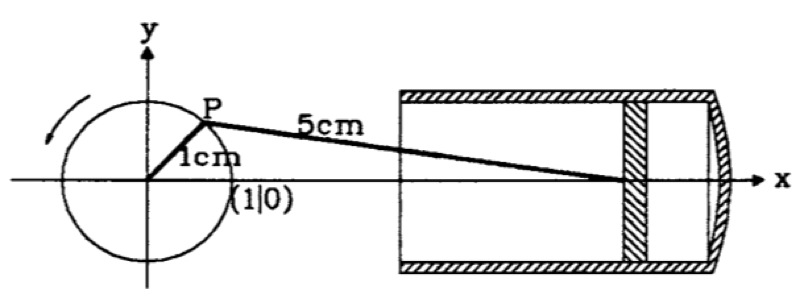
\includegraphics[width=8cm]{pictures/kolben}
\end{center}
\caption{Schema des Kolben}
\end{figure}

Wie schnell bewegt sich der Kolben zu den Zeiten $t=\frac{1}{40}$ und $t=\frac{1}{20}$ Sekunden?
\end{ueb}

\begin{ueb}[sin cos]
\ \\[-4ex]
\begin{enumeratea}
\item Wo und unter welchem Winkel (Schnittwinkel der Tangenten im Schnittpunkt) schneiden sich die Graphen der Sinus- und der Cosinusfunktion im Intervall $[0,\frac{\pi}{2}]$?
\item Wo haben die Graphen die gleiche Steigung im Intervall $[0,2\pi]$?
\end{enumeratea}
\end{ueb}

\subsection{Die Ableitung der Exponentialfunktion}

Um die Ableitung der Exponentialfunktion $\exp(x)=\mathrm{e}^x$ zu bestimmen, muss man den Grenzwert
$$\left(\mathrm{e}^x\right)'=\lim_{h\to0}\frac{\mathrm{e}^{x+h}-\mathrm{e}^x}{h}$$
untersuchen.
\begin{ueb}[wie in der Quarta]
\"Uberzeuge dich davon, dass obiger Grenzwert gleich
$$\mathrm{e}^x\cdot\lim_{h\to0}\frac{\mathrm{e}^h-1}{h}$$
ist.
\end{ueb}
Berechnet man N\"aherungswerte f\"ur den Grenzwert (kleine $h$) mit dem Taschenrechner, so dr\"angt sich die Vermutung
$$\lim_{h\to0}\frac{\mathrm{e}^h-1}{h}=1$$
auf. Dies w\"urde bedeuten, dass die Ableitung der $\mathrm{e}$-Funktion just wieder die $\mathrm{e}$-Funktion ist:
$$\left(\mathrm{e}^x\right)'\stackrel{?}{=}\mathrm{e}^x$$

Wir m\"ussen uns an dieser Stelle mit einer anschaulichen Herleitung begn\"ugen:
F\"ur $h<1$ gilt
$$1+h\leq \mathrm{e}^h\leq\frac{1}{1-h}$$
\begin{center}
\begin{tikzpicture}[line cap=round,line join=round,>=triangle 45,x=1.5cm,y=1.1cm]
\draw[->,color=black] (-2.1,0) -- (2.2,0);
\foreach \x in {-2,-1,1,2}
\draw[shift={(\x,0)},color=black] (0pt,2pt) -- (0pt,-2pt);
\draw[color=black] (2,0.1) node [anchor=south west] { x};
\draw[->,color=black] (0,-0.5) -- (0,3.9);
\foreach \y in {,1,2,3}
\draw[shift={(0,\y)},color=black] (2pt,0pt) -- (-2pt,0pt);
\draw[color=black] (0.04,3.8) node [anchor=west] { y};
\clip(-2.04,-0.44) rectangle (2.12,3.91);
\draw[smooth,samples=100,domain=-2.1:2.12] plot(\x,{1+\x});
\draw[smooth,samples=100,domain=0:2.12] plot(\x,{2.71^(\x)});
\draw[smooth,samples=100,domain=-2.1:-0.01] plot(\x,{1/(2.71^\x)});
\draw[smooth,samples=100,domain=-2.01:0.93] plot(\x,{1/(1-(\x))});
\draw (-0.3,1.3) node[anchor=north west] {$1$};
\draw[color=black] (1,1.5) node {\small$x+1$};
\draw[color=black] (1.3,3) node {$\mathrm{e}^x$};
\draw[color=black] (-1.4,0.7) node {$\frac{1}{1-x}$};
\end{tikzpicture}
\end{center}
also
$$h\leq \mathrm{e}^h-1\leq\frac{1}{1-h}-1=\frac{h}{1-h}$$
Es folgt f\"ur $h>0$
$$1\leq\frac{\mathrm{e}^h-1}{h}\leq\frac{1}{1-h},\text{ also }\lim_{h\downarrow0}\frac{\mathrm{e}^h-1}{h}=1$$
und f\"ur $h<0$
$$1\geq\frac{\mathrm{e}^h-1}{h}\geq\frac{1}{1-h},\text{ also }\lim_{h\uparrow0}\frac{\mathrm{e}^h-1}{h}=1$$
Insgesamt
$$\lim_{h\to0}\frac{\mathrm{e}^h-1}{h}=1$$
\begin{csatz}[exp ist exp]{satz:exp}
Die
\marginnote{
\qrcode{
https://www.youtube.com/watch?v=MkQ55zu9mEM}
}
Exponentialfunktion $\exp(x)=\mathrm{e}^x$ ist f\"ur alle $x\in\mR$ differenzierbar, und es gilt
$$\left(\mathrm{e}^x\right)'=\mathrm{e}^x$$
\end{csatz}

\begin{bem}
F\"ur einen exakten Beweis im mathematischen Sinn m\"usste man zun\"achst die folgenden Eigenschaften zeigen:
\begin{itemize}
\item $\forall x\in\mR\text{ ist }\mathrm{e}^x=\lim_{n\to\infty}\left(1+\frac{x}{n}\right)^n$
\item $<\left(1+\frac{x}{n}\right)^n>$ ist f\"ur $n>\abs{x}$ monoton wachsend
\end{itemize}
also gilt $\left(1+\frac{x}{n}\right)^n\leq \mathrm{e}^x$.

Mit Hilfe der Bernoulli'schen Ungleichung erh\"alt man dann die beiden Ungleichungen
$$1+x=1+n\frac{x}{n}\leq\left(1+\frac{x}{n}\right)^n\leq \mathrm{e}^x,$$
also $1+x\leq \mathrm{e}^x$ und, wenn man $x$ durch $-x$ ersetzt, $1-x\leq \mathrm{e}^{-x}=\frac{1}{\mathrm{e}^x}$.
Aus der zweiten Ungleichung ergibt sich f\"ur $1-x>0$ also
$\mathrm{e}^x\leq\frac{1}{1-x}.$
Damit gilt f\"ur $x<1$: 
$1+x\leq \mathrm{e}^x\leq\frac{1}{1-x}.$
\end{bem}

\subsection{Die Ableitung der Logarithmusfunktion}
F\"ur
\marginnote{
\qrcode{
https://www.youtube.com/watch?v=HczWnwIKa4A}
}
die Herleitung erinnern wir uns an die Inversfunktion der Exponentialfunktion $\mathrm{e}^x$, den nat\"urlichen Logarithmus $\ln(x)$. Allgemein gilt f\"ur eine Funktion $f$ und ihre Inverse $f^{-1}$:
$$f(f^{-1}(x))=f^{-1}(f(x))=x.$$
Wenden wir diese Beziehung auf $\exp$ und $\ln$ an --- und ber\"ucksichtigen, dass $\ln$ nur f\"ur positive Argumente definiert ist --- haben wir
$$\mathrm{e}^{\ln(x)}=x$$
Beide Seiten der Gleichung abgeleitet ergibt:
$$\mathrm{e}^{\ln(x)}\cdot(\ln(x))'=1$$
und daraus folgt unmittelbar
$$(\ln(x))'=\frac{1}{x}.$$
\begin{csatz}[Ableitung ln]{satz:ln}
Die
\marginnote{
\qrcode{
https://www.youtube.com/watch?v=soVDopFBghg}
}
Logarithmusfunktion $\ln(x)$ ist f\"ur alle $x\in\mR^+$ differenzierbar und es gilt
$$(\ln(x))'=\frac{1}{x}.$$
\end{csatz}

\begin{ueb}[ueb again]
Ermittle die Definitionsmenge und die Ableitung der Funktion ($\mapsto$ bedeutet: \glqq wird zugeordnet\grqq)

\begin{minipage}{0.4\textwidth}
\begin{enumeratea}
\item $x\mapsto7\ln(x)$
\item $x\mapsto(\ln(x))^2$
\item $x\mapsto\ln(x-5)$
\item $x\mapsto\ln(\ln(x))$
\item $x\mapsto\sqrt{\ln(x)}$
\item $x\mapsto\ln(\sin(x))$
\end{enumeratea}
\end{minipage}
\begin{minipage}{3.9cm}
\begin{enumeratea}
\addtocounter{enumi}{6}
\item $x\mapsto 3\mathrm{e}^{x}$
\item $x\mapsto \mathrm{e}^{3x}$
\item $t\mapsto 6\mathrm{e}^{-5t+2}$
\item $t\mapsto \mathrm{e}^{2t^4-1}$
\item $t\mapsto \sqrt{t}\mathrm{e}^{\sqrt{t}}$
\item $\chi\mapsto \mathrm{e}^{-\chi^2}\ln(\chi)$
\end{enumeratea}
\end{minipage}
\end{ueb}

\begin{ueb}[Insekten]
Bei einem Experiment mit gleicher Anzahl M\"annchen und Weibchen einer bestimmten Insektenart wurde die Anzahl $N(T)$ Paarungen in Abh\"angigkeit der Temperatur $T$ (in Grad Celsius) beobachtet. Es ergab sich der Funktionsterm
$$N(T)=(0.1T+1)\cdot\ln(\sqrt{T})$$
Berechne die Anzahl Paarungen und die lokale \"Anderungsrate f\"ur $15^\circ C$.
\end{ueb}

\section{Graphenanalyse}

\subsection{Extrema}

\begin{cdef}[Extrema]{def:extrema}
Der Punkt $(x_0|f(x_0))$ heisst \emph{relatives Minimum} oder Tiefpunkt, falls
$$f(x)>f(x_0)$$
f\"ur alle $x$ in einer hinreichend kleinen Umgebung von $x_0$.
\begin{center}
\definecolor{xdxdff}{rgb}{0.49,0.49,1}
\scalebox{0.9}{
\begin{tikzpicture}[line cap=round,line join=round,>=triangle 45,x=0.8cm,y=0.8cm]
\draw[->,color=black] (-0.48,0) -- (8.9,0);
\foreach \x in {,1,2,3,4,5,6,7,8}
\draw[shift={(\x,0)},color=black] (0pt,2pt) -- (0pt,-2pt);
\draw[color=black] (8.56,0.08) node [anchor=south west] {$x$};
\draw[->,color=black] (0,-0.86) -- (0,4.36);
\foreach \y in {,1,2,3,4}
\draw[shift={(0,\y)},color=black] (2pt,0pt) -- (-2pt,0pt);
\draw[color=black] (0.1,3.96) node [anchor=west] {$y$};
\clip(-0.48,-0.86) rectangle (8.9,4.36);
\draw[smooth,samples=100,domain=0.3:7.5] plot(\x,{0.1*(\x-5)^2+1.5});
\draw [dotted] (5,1.5)-- (5,0);
\draw (3.9,2.5) node[anchor=north west] {Minimalpunkt};
\draw (4.72,-0.14) node[anchor=north west] {$x_0$ (Extremalstelle)};
\draw (0.7,1) node[anchor=north west] {Minimum (Extremwert)};
\fill [color=xdxdff] (5,1.5) circle (1.5pt);
\end{tikzpicture}
}
\end{center}
$(x_0|f(x_0))$ heisst \emph{relatives Maximum} oder Hochpunkt, falls
$$f(x)<f(x_0)$$
f\"ur alle $x$ in einer hinreichend kleinen Umgebung von $x_0$.
\begin{center}
\definecolor{xdxdff}{rgb}{0.49,0.49,1}
\scalebox{0.9}{
\begin{tikzpicture}[line cap=round,line join=round,>=triangle 45,x=0.8cm,y=0.8cm]
\draw[->,color=black] (-0.48,0) -- (8.9,0);
\foreach \x in {,1,2,3,4,5,6,7,8}
\draw[shift={(\x,0)},color=black] (0pt,2pt) -- (0pt,-2pt);
\draw[color=black] (8.56,0.08) node [anchor=south west] { $x$};
\draw[->,color=black] (0,-0.86) -- (0,4.36);
\foreach \y in {,1,2,3,4}
\draw[shift={(0,\y)},color=black] (2pt,0pt) -- (-2pt,0pt);
\draw[color=black] (0.1,3.96) node [anchor=west] {$y$};
\clip(-0.48,-0.86) rectangle (8.9,4.36);
\draw[smooth,samples=100,domain=0.4:6.0] plot(\x,{0-(0.2)*(\x-4)^2+3});
\draw [dotted] (4,3)-- (4,0);
\draw (2.96,3.7) node[anchor=north west] {Maximalpunkt};
\draw (3.7,1.64) node[anchor=north west] {Maximum (Extremalwert)};
\draw (3.62,-0.3) node[anchor=north west] {$x_0$ (Extremalstelle)};
\fill [color=xdxdff] (4,3) circle (1.5pt);
\end{tikzpicture}
}
\end{center}
\end{cdef}

\clearpage

Wie man diese Punkte rechnerisch findet, beschreiben die folgenden beiden S\"atze.
\begin{csatz}{satz:extremum}
Hat
\marginnote{
\qrcode{
https://www.youtube.com/watch?v=VloOTGZ8SGQ}
}
die Funktion $f$ im Punkt $x_0$ ein relatives Minimum oder Maximum, dann gilt
$$f'(x_0)=0.$$
\end{csatz}
Beachten Sie, dass diese Bedingung f\"ur eine Extremalstelle notwendig, aber nicht hinreichend, ist. Um zu entscheiden, ob sich im Punkt $x_0$ ein Minimum oder Maximum befindet, hilft der folgende
\begin{csatz}{satz:kruemmung}
Ist $f''(x_0)>0$, dann ist der Graph von $f$ dort linksgekr\"ummt. Ist $f''(x_0)<0$, dann ist der Graph von $f$ dort rechtsgekr\"ummt.
\end{csatz}
Zusammengefasst heisst dies, dass wenn $f$ ein Minimum in $x_0$ hat, dort $f'(x_0)=0$ und $f''(x_0)>0$ ist, und wenn $f$ ein Maximum in $x_0$ hat, dass $f'(x_0)=0$ und $f''(x_0)<0$.

\subsection{Wendepunkte}
Das letzte Resultat wirft die Frage auf, wie ein Punkt $x_0$ von $f$ interpretiert werden soll, falls dort $f'(x_0)=0$ und $f''(x_0)=0$ ist. Wenn wir uns daran erinnern, dass die erste Ableitung einer Funktion die Steigung und die zweite Ableitung die Kr\"ummung in einer hinreichend kleinen Umgebung von $x_0$ angibt, dann bedeutet $f''(x_0)=0$ also, dass dort der Graph von $f$ keine Kr\"ummung besitzt.

\begin{cdef}[Terrassenpunkt]{def:terrasse}
Man nennt einen Punkt $(x_0|f(x_0))$ \emph{Terrassenpunkt} von $f$, falls $f'(x_0)=0$, $f''(x_0)=0$ und $f'''(x_0)\neq0$ gilt.
\end{cdef}

\begin{center}
\definecolor{uququq}{rgb}{0.25,0.25,0.25}
\begin{tikzpicture}[line cap=round,line join=round,>=triangle 45,x=0.8cm,y=0.8cm]
\draw[->,color=black] (-0.48,0) -- (8.12,0);
\foreach \x in {,1,2,3,4,5,6,7}
\draw[shift={(\x,0)},color=black] (0pt,2pt) -- (0pt,-2pt);
\draw[color=black] (7.78,0.08) node [anchor=south west] {$x$};
\draw[->,color=black] (0,-0.72) -- (0,4.36);
\foreach \y in {,1,2,3,4}
\draw[shift={(0,\y)},color=black] (2pt,0pt) -- (-2pt,0pt);
\draw[color=black] (0.1,3.96) node [anchor=west] {$y$};
\clip(-0.48,-0.72) rectangle (8.12,4.36);
\draw[smooth,samples=100,domain=0.3:7.0] plot(\x,{0.1*(\x-3.5)^3+2});
\draw [dash pattern=on 3pt off 3pt] (0.46,2)-- (6.6,2);
\draw [dotted] (3.5,2)-- (3.5,0);
\draw (3.2,0) node[anchor=north west] {$x_0$};
\draw (1.4,2.6) node[anchor=north west] {Terrassenpunkt};
\draw[color=black] (0.74,-0.48) node {$f$};
\fill [color=uququq] (3.5,2) circle (1.5pt);
\end{tikzpicture}
\end{center}
Schliesslich will ich noch einen letzten Begriff zur Kurvendiskussion einf\"uhren, den sogenannten \emph{Wendepunkt}. Man spricht dann von einem Wendepunkt von $f$ an der Stelle $x_0$, wenn $f''(x_0)=0$ und $f'''(x_0)\neq0$.
\begin{bem}
Ein Terrassenpunkt ist also ein spezieller Wendepunkt, n\"amlich ein Wendepunkt mit Horizontaltangente.
\end{bem}

\subsection{\"Uberblick}
\marginnote{
\qrcode{
https://www.youtube.com/watch?v=X6RepNNUTLw}
}
\begin{itemize}
\item Hat $f$ an der Stelle $x_0$ ein Extremum, dann gilt
$$f'(x_0)=0$$
\item Hat $f$ an der Stelle $x_0$ einen Wendepunkt, dann gilt
$$f''(x_0)=0$$
\item Gilt $f'(x_0)=0$ und $f''(x_0)\neq0$, dann hat $f$ an der Stelle $x_0$ ein Extremum, und zwar
\begin{itemize}
\item ein Maximum, falls
$$f''(x_0)<0$$
\item ein Minimum, falls
$$f''(x_0)>0$$
\end{itemize}
\item Gilt $f''(x_0)=0$ und $f'''\neq0$, dann hat $f$ einen Wendepunkt in $x_0$.
\end{itemize}

\begin{bem}
Die Umkehrung dieser S\"atze gilt nicht.
\end{bem}

\begin{ueb}[gegenbsp]
\"Uberpr\"ufe obige Aussage anhand einfacher Gegenbeispiele. Betrachte
$$f(x)=x^3\q\text{und}\q g(x)=x^4$$
in $x_0=0$.
\end{ueb}

\begin{ueb}[quadrfkt]
 Zeige, dass eine beliebige quadratische Funktion keinen Wendepunkt hat.
 \end{ueb}
 \begin{ueb}[polynomfkt]
 Bestimme die Nullstellen, Extrema und Wendepunkte der Funktion
 $$f(x) = x^3-2x^2-5x+6.$$
 Zeige zuerst, dass bei $x=1$ eine Nullstelle ist und wende anschliessend Polynomdivision an, um die restlichen zu finden.
 \end{ueb}

\begin{ueb}[selber mit geogebra]
Gib dir eine ganzrationale Funktion vor (z.B. $f(x)=4x^3-3x+1$) und untersuche diese nach Nullstellen, Symmetrie, Extrema und Wendepunkte. \"Uberpr\"ufe deine Berechnungen z.B. mit GeoGebra.
\end{ueb}

\begin{ueb}[sin analysiert]
Zeichne die Sinusfunktion
$$f(x) = \sin{x}$$
im Intervall $[-4\pi,4\pi]$. Gib danach f\"ur $f$ Nullstellen, Symmetrie, Extrema und Wendepunkte auf dem Definitionsbereich $\D{D}=\D{R}$ an. Zeichne mit einer andern Farbe ins gleiche Koordinatensystem die erste und zweite Ableitung von $f$ ein.
\end{ueb}

\begin{ueb}[drosophila melanogaster]
Die Vermehrungsrate von drosophila melanogaster ist stark fallend, wenn die Populationsdichte zunimmt. Es seien $x$ die Anzahl Fliegen pro Flasche und $f(x)$ die Anzahl Nachkommen eines Weibchens pro Tag. Empirisch wurde gefunden, dass
$$f(x) =34.53\cdot \mathrm{e}^{-0.018x}x^{-0.658}$$
Berechne $f(20)$ und $f'(20)$.
\end{ueb}

\clearpage

\begin{ueb}[Glockenkurve]
Die
\marginnote{
\qrcode{
https://www.youtube.com/watch?v=rfXO1n9Av3I}
}
Funktion
$$g(x)=\mathrm{e}^{-x^2}$$
spielt in der Wahrscheinlichkeitsrechnung und Statistik eine beherrschende Rolle im Zusammenhang mit der Normal- oder Gauss'schen Verteilung. Ermittle
\begin{enumeratea}
\item Definitions- und Wertemenge,
\item $\lim_{x\to\pm\infty}f(x)$
\item Maxima und Minima,
\item Wendepunkte des Graphen.
\item Skizzieren Sie den glockenf\"ormigen Graphen von $f$ mit den Informationen aus dieser \"Ubung.
\item Zeige, dass $g$ symmetrisch zur $y$-Achse ist.
\end{enumeratea}
\end{ueb}

\clearpage

\section{Extremwertaufgaben}
\begin{wrapfigure}{r}{0.382\textwidth}
\vspace{-22pt}
  \begin{center}
    
\includegraphics[width=0.382\textwidth]{pictures/can}
  \end{center}
%\caption{You Know my Name}
\vspace{-10pt}
\end{wrapfigure}
Bei der Evolution haben sich alle Funktionen eines Organismus, soweit sie wesentlich zum \"Uberleben sind, optimal entwickelt. Die dazu n\"otige Energie sollte nach M\"oglichkeit minimal sein. Bl\"atter und Pflanzen sollten m\"oglichst viel Sonnenlicht erhalten, die Wurzeln sollten mit m\"oglichst vielen lebenswichtigen Mineralien Kontakt haben. Wild lebende Tiere m\"ussen sich m\"oglichst gut gegen ihre Feinde sch\"utzen k\"onnen und gute Nahrungsbeschaffer sein. Die Empfindlichkeit eines Organismus bez\"uglich Krankheiten sollte auf ein Minimum reduziert werden.

So wie bei den obigen Beispielen aus der Natur begegnet man in unserer Umwelt sehr oft gewissen Gr\"ossen, die entweder zu minimieren (Kosten, Zeiten, Kraftaufwand,\dots) oder zu maximieren (Gewinne, Ausnutzung, Nutzeffekt,\dots) sind. Handelt es sich dabei um mehrere Variablen, die durch lineare Ungleichungen miteinander verbunden sind, so konnten diese Aufgaben mathematisch mit der linearen Optimierung gel\"ost werden. Im folgenden l\"asst sich der reale Zusammenhang durch eine differenzierbare Funktion mit nur einer Variablen beschreiben. Die Differenzialrechnung liefert dann mit ihren Methoden der Extremwertermittlung die L\"osung des gestellten Problems.

\begin{bem}
Bei manchen Problemstellungen können \emph{Randextrema} vorkommeb: Mit den Bezeichnungen aus Abbildung \ref{randextrem} auf Seite \pageref{randextrem} erreicht im Punkte $R$ die Funktion ihr globales Maximum (Randextremum). Im Punkt $Q$ erreicht sie ein lokales Maximum, w\"ahrend sie in $P$ sowohl ein globales als auch ein lokales Minimum erreicht.

\begin{figure}
\begin{center}
\definecolor{uququq}{rgb}{0.25,0.25,0.25}
\definecolor{xdxdff}{rgb}{0.49,0.49,1}
\scalebox{0.9}{
\begin{tikzpicture}[line cap=round,line join=round,>=triangle 45,x=0.7cm,y=0.7cm]
\draw[->,color=black] (-0.56,0) -- (9.07,0);
\foreach \x in {,2,4,6,8}
\draw[shift={(\x,0)},color=black] (0pt,2pt) -- (0pt,-2pt);
\draw[color=black] (8.73,0.08) node [anchor=south west] {$x$};
\draw[->,color=black] (0,-0.88) -- (0,4.36);
\foreach \y in {,2,4}
\draw[shift={(0,\y)},color=black] (2pt,0pt) -- (-2pt,0pt);
\draw[color=black] (0.1,3.95) node [anchor=west] {$y$};
\clip(-0.56,-0.88) rectangle (9.07,4.36);
\draw[smooth,samples=100,domain=0.2:8.0] plot(\x,{0-(0.03)*(\x-5)^3+0.3*\x});
\draw [dotted] (0.44,2.98)-- (0.44,0.02);
\draw [dotted] (7.81,1.68)-- (7.81,0);
\draw (0.2,0.05) node[anchor=north west] {$a$};
\draw (7.6,0.05) node[anchor=north west] {$b$};
\fill [color=xdxdff] (0.44,2.98) circle (1.5pt);
\draw[color=xdxdff] (0.6,3.4) node {$R$};
\fill [color=uququq] (3.17,1.13) circle (1.5pt);
\draw[color=uququq] (3.4,1.5) node {$P$};
\fill [color=uququq] (6.83,1.87) circle (1.5pt);
\draw[color=uququq] (6.99,2.2) node {$Q$};
\end{tikzpicture}
}
\end{center}
\caption{Randextremwert}\label{randextrem}
\end{figure}
\end{bem}

\begin{ueb}[Normgewicht]
F\"ur normalgewichtige Schweizer (0\% \"Ubergewicht, 0\% Untergewicht) betr\"agt die Lebenserwartung 72.3 Jahre. Diese Zahl beruht auf Erfahrungen aus den Jahren 1978-1983. Durch Untersuchungen an M\"annern mit $x\%$ Unter- bzw. \"Ubergewicht ergab sich die f\"ur das Intervall $-20\%\leq x\% \leq 20\%$ g\"ultige Lebenserwartungsfunktion
$$L(x)=72-0.035x^2-0.7x$$
Wann ist die Lebenserwartung maximal? Wie hoch ist sie?
\end{ueb}

\begin{ueb}[zerlegen]
Zerlege die Zahl 144 so in zwei Summanden, dass
\begin{enumeratea}
\item ihr Produkt m\"oglichst gross,
\item die Summe ihrer Quadrate m\"oglichst klein wird.
\end{enumeratea}
\end{ueb}

\begin{ueb}[Parabel]
Zeichne in einem Koordinatensystem die Parabel mit der Gleichung
$$f(x) = 6 - \frac{x^2}{4}$$
Dem Abschnitt der Parabel, der oberhalb der $x$-Achse liegt, ist ein Rechteck mit m\"oglichst grossem
\begin{enumeratea}
\item Inhalt,
\item Umfang
\end{enumeratea}
einzubeschreiben.
\end{ueb}

\begin{ueb}[Stau]
Ein Auto beansprucht in einem Tunnel mindestens einen Strassenabschnitt der L\"ange $L+s_R+s_B$, wobei $L$ der durchschnittlichen L\"ange eines Autos, $s_R=tv$ dem Reaktionsweg, $s_B=\frac{v^2}{2a}$ dem Bremsweg, also $s_R+s_B$ dem Anhalteweg entsprechen. ($a$: Bremsverz\"ogerung, $t$: Reaktionszeit, $v$: Momentangeschwindigkeit)
Ein Stau vor dem Tunnel kann am schnellsten abgebaut werden, wenn ein maximaler Autodurchfluss im Tunnel erzeugt wird. Der Autodurchfluss $D$ wird durch die Anzahl Autos, die pro Stunde maximal in den Tunnel einfahren k\"onnen, definiert:
$$D(v):=\frac{3600v}{L+tv+\frac{v^2}{2a}}$$
\begin{enumeratea}
\item F\"ur welche Geschwindigkeit wird dieser Durchfluss maximal? Wie viele Autos k\"onnen pro Stunde in den Tunnel einfahren? (Realistische Werte: $L=\unit[5]{m}, a=\unitfrac[5]{m}{s^2}, t=\unit[1.2]{s}$)

{\small Hinweis: Statt des Maximums von $D$ kann einfacher das Minimum von $\frac{1}{D}$ ermittelt werden.}
\item Wie \"andert sich das Resultat, wenn die Reaktionszeit sich \"andert, die Fahrzeugl\"ange sich vergr\"ossert, gute Bremsen ($a=\unitfrac[8]{m}{s^2}$) vorhanden sind?
\end{enumeratea}
\end{ueb}

\begin{ueb}[Heizkessel]
 Ein Heizkessel besteht aus einem Zylinder mit aufgesetzter Halbkugel. Er soll $\unit[2000]{Liter}$ fassen und m\"oglichst wenig W\"arme abstrahlen. Berechne seine Höhe und den Radius des Zylinders bzw. der Halbkugel.
 \end{ueb}

\begin{ueb}[Büchse]
Eine
\marginnote{
\qrcode{
https://www.youtube.com/watch?v=6kFezQk7R-0}
}
kreiszylinderf\"ormige B\"uchse hat den Inhalt $\unit[1]{l}$. Welche Abmessungen hat diese B\"uchse, wenn ihre Oberfl\"ache, bestehend aus Mantel und Grundfl\"ache, minimal werden soll?
\end{ueb}

\begin{ueb}[Marktpreis]
Der Marktpreis f\"ur ein Buch, von dem $x$ Exemplare hergestellt werden sollen, wird durch
$$p(x)=2500-\frac{x}{10}$$
angegeben. Die Kosten des Verlegers betragen
$$K(x)=4000+6x+0.00084x^2$$
Dem Autor wurde eine Umsatzbeteiligung von 20\% zugesprochen. Welche Preis-Mengen-L\"osung bevorzugt der Verleger (Gewinnmaximierung), welche der Autor (Umsatzmaximierung)? Gibt es einen Unterschied.
\end{ueb}

\begin{ueb}[Drogen]
Die
\marginnote{
\qrcode{
https://www.youtube.com/watch?v=mpG6fCreiQQ}
}
Funktion
$$f(t)=c\left(\mathrm{e}^{-at}-\mathrm{e}^{-bt}\right)$$
mit $c>0, b>a>0, t\geq0$ wird gebraucht, um die Konzentration einer Drogeninjektion in die Blutbahn in Abh\"angigkeit der Zeit t zu beschreiben.
\begin{enumeratea}
\item \"Uberpr\"ufe den Funktionsterm f\"ur $t = 0$ und zeige,
dass $f(t) >0$ f\"ur $t >0$ ist.
\item Zu welchem Zeitpunkt (in Abh\"angigkeit der drei Parameter a, b und c) erreicht die Konzentration ihr Maximum?
\end{enumeratea}
\end{ueb}

\begin{ueb}[gedämpfte Schwingung]
Durch
\marginnote{
\qrcode{
https://www.youtube.com/watch?v=mMQ1X1s0Pa8}
}
die Funktionen vom Typ
$$f(t)=A\mathrm{e}^{-\ga t}\sin(\go t)$$
mit $t>0$ lassen sich Schwingungen beschreiben, die durch nicht zu starke Reibung abgebremst werden. Der Faktor $A\sin(\go t)$ entspricht der unged\"ampften Schwingung, w\"ahrend der Faktor $\mathrm{e}{-\ga t}$ mit der positiven Konstanten $\ga$ f\"ur die Abnahme der Amplitude sorgt. Berechne das erste Maximum und das erste Minimum der Funktion, falls $A = 1$, $a = 0.3$ und $\go=2$.
\end{ueb}

\begin{ueb}[Mühle]
In einer alten M\"uhle soll ein Kaffee er\"offnet werden. Den zylinderf\"ormigen Wassertank, der im kegelf\"ormigen Dach untergebracht wird, will man so bauen, dass sein Volumen m\"oglichst gross wird. Der Durchmesser des Dachs betr\"agt $\unit[3]{m}$ und die H\"ohe $\unit[2.5]{m}$. Wie m\"ussen die Abmessungen des Tanks gew\"ahlt werden und welches Volumen fasst er?\\[3ex]

\begin{center}
\definecolor{qqzzqq}{rgb}{0,0.6,0}
\definecolor{qqqqcc}{rgb}{0,0,0.8}
\definecolor{ffqqqq}{rgb}{1,0,0}
\definecolor{zzttqq}{rgb}{0.6,0.2,0}
\definecolor{uququq}{rgb}{0.25,0.25,0.25}
\scalebox{1.4}{
\begin{tikzpicture}[line cap=round,line join=round,>=triangle 45,x=1.3cm,y=1.3cm]
\draw[->,color=uququq] (-3.27,0) -- (2.61,0);
\foreach \x in {-3,-2,-1,1,2}
\draw[shift={(\x,0)},color=uququq] (0pt,2pt) -- (0pt,-2pt);
\draw[->,color=uququq] (0,-0.5) -- (0,2.9);
\foreach \y in {,1,2}
\draw[shift={(0,\y)},color=uququq] (2pt,0pt) -- (-2pt,0pt);
\clip(-3.27,-0.5) rectangle (2.61,2.9);
\fill[color=zzttqq,fill=zzttqq,fill opacity=0.1] (-3,0) -- (0,0) -- (-1.5,2.5) -- cycle;
\fill[color=qqqqcc,fill=qqqqcc,fill opacity=0.1] (-2.72,0) -- (-2.72,0.46) -- (-0.28,0.46) -- (-0.28,0) -- cycle;
\draw [color=zzttqq] (-3,0)-- (0,0);
\draw [color=zzttqq] (0,0)-- (-1.5,2.5);
\draw [color=zzttqq] (-1.5,2.5)-- (-3,0);
\draw [color=qqqqcc] (-2.72,0)-- (-2.72,0.46);
\draw [color=qqqqcc] (-2.72,0.46)-- (-0.28,0.46);
\draw [line width=2pt,color=qqqqcc] (-0.28,0.46)-- (-0.28,0);
\draw [color=qqqqcc] (-0.28,0)-- (-2.72,0);
\draw [line width=2pt,color=ffqqqq] (-1.5,0)-- (-0.28,0);
\draw [dash pattern=on 3pt off 3pt,color=qqzzqq] (1.22,2.17)-- (1.22,0);
\draw [line width=1.2pt,dash pattern=on 5pt off 5pt] (-1.5,2.5)-- (-1.5,0);
\draw [line width=2pt,color=ffqqqq] (0,0)-- (1.22,0);
\draw [color=zzttqq](-3.2,2.47) node[anchor=north west] {M\"uhledach};
\draw [color=qqqqcc](-2.5,0.8) node[anchor=north west] {Wasserbeh\"alter};
\draw [color=ffqqqq](0.75,-0.17) node[anchor=north west] {r = 1.22};
\draw [color=qqzzqq](1.35,1.21) node[anchor=north west] {V = 2.17};
\draw [color=qqzzqq](0.06,2.77) node[anchor=north west] {Volumen};
\fill [color=uququq] (-1.5,0) circle (1.0pt);
\fill [color=ffqqqq] (-0.28,0) circle (2.0pt);
\draw[color=qqqqcc] (-0.8,0.22) node {$h = 0.46$};
\draw[color=ffqqqq] (-0.86,-0.23) node {$r = 1.22$};
\fill [color=qqzzqq] (1.22,2.17) circle (1.5pt);
\end{tikzpicture}
}
\end{center}
\end{ueb}

\newpage

\appendix

\section{Klassiker Tetrapack}

\begin{ueb}
Abschliessend
\marginnote{
\qrcode{
https://www.youtube.com/watch?v=0HnulX11-DQ}
}
zu Extremalaufgaben wollen wir untersuchen, ob die Liter-Milchbeutel optimale Abmessungen haben, das heisst bei zur Verf\"ugung stehendem Verpackungsmaterial den gr\"osstm\"oglichen Volumeninhalt aufweisen. Wir werden dabei auf ein Ergebnis stossen, dass uns auf den ersten Blick erstaunen mag.

\begin{center}
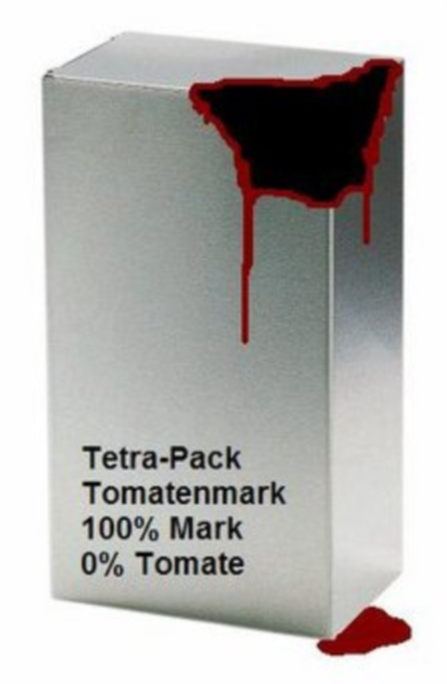
\includegraphics[width=0.618\textwidth]{pictures/Tetrapack}
\end{center}
\end{ueb}

\newpage

\subsection{Symmetrie}
Wir unterscheiden zwei Arten von Symmetrien, die bei Graphen von Funktionen auftauchen k\"onnen. Diese Charakterisierungen gelten f\"ur Funktionen allgemein, nicht bloss f\"ur ganzrationale Funktionen.
\subsubsection{Achsialsymmetrie bez\"uglich y-Achse}
\begin{csatz}{satz:achsialsym}
Der Graph einer Funktion $f$ ist genau dann achsialsymmetrisch zur y-Achse, wenn
$$f(-x) = f(x)$$
f\"ur alle $x\in\D{D}$ gilt.
\end{csatz}
\begin{proof}[Beweis]
Man veranschauliche sich den Sachverhalt an einem kleinen Bildchen.
\end{proof}

\begin{figure}[h!]
\begin{center}
\definecolor{xdxdff}{rgb}{0.49,0.49,1}
\definecolor{qqqqff}{rgb}{0,0,1}
\scalebox{0.618}{
\begin{tikzpicture}[line cap=round,line join=round,>=triangle 45,x=0.5cm,y=0.5cm]
\draw[->,color=black] (-5.9,0) -- (6.3,0);
\foreach \x in {-5,-4,-3,-2,-1,1,2,3,4,5,6}
\draw[shift={(\x,0)},color=black] (0pt,2pt) -- (0pt,-2pt);
\draw[color=black] (5.96,0.08) node [anchor=south west] {$x$};
\draw[->,color=black] (0,-3) -- (0,7.5);
\foreach \y in {-2,-1,1,2,3,4,5,6,7}
\draw[shift={(0,\y)},color=black] (2pt,0pt) -- (-2pt,0pt);
\draw[color=black] (0.1,7.02) node [anchor=west] {$y$};
\clip(-5.84,-3) rectangle (6.3,7.5);
\draw[line width=1.6pt, smooth,samples=100,domain=-5.84:6.3] plot(\x,{0.5*(\x*\x)-2});
\draw [dotted] (-4,6)-- (-4,0);
\draw [dotted] (4,0)-- (4,6);
\draw [dotted] (-4,6)-- (4,6);
\draw (-4.7,0) node[anchor=north west] {$-x$};
\draw (3.6,0) node[anchor=north west] {$x$};
\draw (4.1,3.4) node[anchor=north west] {$f(x)$};
\draw (-6.1,3.4) node[anchor=north west] {$f(-x)$};
\draw[color=black] (-5,7) node {$f$};
\fill [color=qqqqff] (4,6) circle (1.5pt);
\fill [color=xdxdff] (-4,6) circle (1.5pt);
\end{tikzpicture}
\definecolor{xdxdff}{rgb}{0.49,0.49,1}
\begin{tikzpicture}[line cap=round,line join=round,>=triangle 45,x=0.5cm,y=0.5cm]
\draw[->,color=black] (-5.8,0) -- (6.34,0);
\foreach \x in {-5,-4,-3,-2,-1,1,2,3,4,5,6}
\draw[shift={(\x,0)},color=black] (0pt,2pt) -- (0pt,-2pt);
\draw[color=black] (6,0) node [anchor=south west] {$x$};
\draw[->,color=black] (0,-4.86) -- (0,5.5);
\foreach \y in {-4,-3,-2,-1,1,2,3,4,5}
\draw[shift={(0,\y)},color=black] (2pt,0pt) -- (-2pt,0pt);
\draw[color=black] (0.1,5.1) node [anchor=west] {$y$};
\clip(-6.5,-5.2) rectangle (6.34,5.5);
\draw[line width=1.6pt, smooth,samples=100,domain=-5.8:6.34] plot(\x,{\x^3/16});
\draw [dotted] (-4,0)-- (-4,-4);
\draw [dotted] (4,0)-- (4,4);
\draw [dotted] (4,4)-- (0,4);
\draw [dotted] (-4,-4)-- (0,-4);
\draw (4.12,2.4) node[anchor=north west] {$f(x)$};
\draw (-6.5,-1.46) node[anchor=north west] {$-f(-x)$};
\draw (-4.8,1) node[anchor=north west] {$-x$};
\draw (3.6,0) node[anchor=north west] {$x$};
\draw[color=black] (-3.72,-4.9) node {$f$};
\fill [color=xdxdff] (-4,-4) circle (1.5pt);
\fill [color=xdxdff] (4,4) circle (1.5pt);
\end{tikzpicture}
}
\end{center}

\caption{Achsensymmetrie bez\"uglich $y$-Achse, Zentralsymmetrie zu Ursprung}
\end{figure}

\subsubsection{Zentralsymmetrie bez\"uglich Ursprung}
\begin{csatz}{satz:punktsym}
Der Graph einer Funktion $f$ ist genau dann punktsymmetrisch zum Ursprung, wenn
$$-f(-x) = f(x)$$
f\"ur alle $x\in\D{D}$ gilt.
\end{csatz}
\begin{proof}[Beweis]
Man veranschauliche sich den Sachverhalt ebenfalls an einem kleinen Bildchen.
\end{proof}

Um das qualitative Verhalten einer Funktion besser zu verstehen, lohnt es sich, ihren Graphen zu betrachten. Dazu m\"usste man die Werte aus einer umfangreichen Wertetabelle in ein Koordinatensystem \"ubertragen. In vielen F\"allen kann man den Graphen schnell skizzieren, wenn man nur einige markante Punkte des Graphen kennt und untersucht, wie sich die Funktionswerte verhalten, falls die $x$-Werte gegen $\infty$ bzw. $-\infty$ streben.

\begin{ueb}[sin cos again]
Nenne eine gerade und eine ungerade Winkelfunktion.
\end{ueb}

\newpage

\section{Mathematik und Wirtschaft}
Die in den Wirtschaftswissenschaften h\"aufig benutzten Funktionen sind
\begin{itemize}
\item Kostenfunktion $K(x)$
\item St\"uckkostenfunktion $k(x)=\frac{K(x)}{x}$
\item Preisfunktion $p(x)$
\item Erl\"osfunktion $E(x)=x\cdot p(x)$
\item Gewinnfunktion $G(x)=E(x)-K(x)$
\item Angebotsfunktion $p_A(x)$
\item Nachfragefunktion $p_N(x)$
\end{itemize}

Ver\"andert man eine Produktion von $x_0$ Einheiten auf $x_1$ Einheiten, so entsteht ein Kostenzuwachs $\gD K$. Der Differenzenquotient
$$\frac{\gD K(x)}{\gD x}=\frac{K(x_1)-K(x_0)}{x_1-x_0}$$
entspricht dem durchschnittlichen Kostenzuwachs.
Wenn die Funktion $K$ differenzierbar ist, gibt der differenzialquotient
$$K'(x_0)=\lim_{h\to0}\frac{K(x_0+h)-K(x_0)}{h}$$
die Grenzkosten, auch marginale Kosten genannt, bei der Produktion von $x_0$ Einheiten an.Durch $K'(x_0)$ erh\"alt man die Produktionskosten f\"ur eine zus\"atzliche Einheit, wenn schon $x_0$ Einheiten produziert werden.
In ganz \"ahnlicher Weise sind marginaler Preis, Grenzerl\"os, Grenznutzen oder Grenzneigung zum Konsum durch Differenzialquotienten definiert. Beispielsweise gibt
$$\frac{dG(x_0)}{\mathrm{d}x}$$
in erster N\"aherung an, um wie viele Einheiten sich der Gewinn ver\"andert, wenn die unabh\"angige Variable, die Ausbringung eines Gutes, sich um eine Einheit, von $x_0$ auf $x_0 + 1$, ver\"andert.

\begin{ueb}
Die Herstellungskosten f\"ur $x$ ME einer Ware ist
gegeben durch die Funktion
$$K(x)=0.02(x-8)^3+12$$
$0<x<18$, $K(x)$ in GE. Die Grenzkostenfunktion gibt bekanntlich an, wie eine \"Anderung der Produktionsmenge auf die Kosten wirkt. Der Hersteller interessiert sich auch f\"ur die Ableitung der Umkehrfunktion. Was gibt sie an? Bezeichnen Sie die Umkehrfunktion von $K$ mit $S$ und berechnen Sie den Funktionsterm von $S$; berechnen Sie $S'(17)$ und interpretieren Sie das Ergebnis.
\end{ueb}

\begin{ueb}
According to classical economic theory, the demand for a commodity in a free market decreases as the price $x$ increases. Suppose that the number $D(x)$ of transistor radios people are willing to buy per week in a given city at a price $x$ \$ is given by
$$D(x)=\frac{50000}{(x+5)^2}$$
$5<x<15$. Find $D'(x)$, the rate of change of demand with
respect to price change. Find $D'(5)$ and $D'(10)$ and interpret.
\end{ueb}

\medskip

\begin{center}
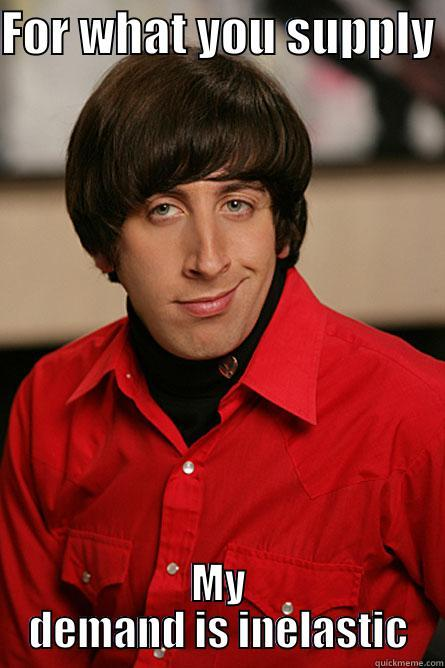
\includegraphics[width=0.382\textwidth]{pictures/inelastic}
\end{center}

\clearpage

\section{Vom Regenbogen}
Manchmal,
\marginnote{
\qrcode{
https://www.youtube.com/watch?v=tdSILv7E7t4}
}
wenn genug Zeit übrig ist, behandle ich noch den Regenbogen als Extremalaufgabe.

\cleardoublepage
\listoffigures
\listoftables
%\newpage
%\nocite{*}
%\bibliographystyle{plain}
%\bibliography{preamble/literaturgoogle}
\end{document}